\documentclass[12pt]{article}

\usepackage{amssymb,amsmath,dsfont,amsfonts,eurosym,geometry,ulem,graphicx,tabularx,booktabs,caption,color,setspace,sectsty,comment,footmisc,caption,natbib,pdflscape,subfigure,array,hyperref}
\usepackage[para,online,flushleft]{threeparttable}
\usepackage{tikz}

\normalem

\onehalfspacing
\newtheorem{theorem}{Theorem}
\newtheorem{corollary}[theorem]{Corollary}
\newtheorem{proposition}{Proposition}
\newenvironment{proof}[1][Proof]{\noindent\textbf{#1.} }{\ \rule{0.5em}{0.5em}}

\newtheorem{hyp}{Hypothesis}
\newtheorem{subhyp}{Hypothesis}[hyp]
\renewcommand{\thesubhyp}{\thehyp\alph{subhyp}}

\newcommand{\red}[1]{{\color{red} #1}}
\newcommand{\blue}[1]{{\color{blue} #1}}

\newcolumntype{L}[1]{>{\raggedright\let\newline\\arraybackslash\hspace{0pt}}m{#1}}
\newcolumntype{C}[1]{>{\centering\let\newline\\arraybackslash\hspace{0pt}}m{#1}}
\newcolumntype{R}[1]{>{\raggedleft\let\newline\\arraybackslash\hspace{0pt}}m{#1}}

\geometry{left=1.0in,right=1.0in,top=1.0in,bottom=1.0in}

\usepackage[toc,title,page]{appendix}

%\providecommand{\addappheadtotoc}{%  no change
\renewcommand{\addappheadtotoc}{%     new simple version
  \phantomsection
  \addcontentsline{toc}{part}{\appendixtocname}%
}

\usepackage{bookmark,hyperref}

\begin{document}

\title{Industrial Policy and Technological Path: The Case of Chinese Solar Photovoltaics Manufacturing Industry}

\author{Dana Golden \and Xiangjun Ma \and  Yiyi Zhou\thanks{Golden: Department of Economics, Stony Brook University, dana.golden@stonybrook.edu. Ma: School of Finance and Trade, Liaoning University, aqj474@gmail.com. Zhou: Department of Economics, Stony Brook University, yiyi.zhou@stonybrook.edu.}}

\maketitle

\begin{abstract}

\singlespacing 

We estimate ...



\thispagestyle{empty}

\begin{description}
\item[Keywords:] 

\item[JEL Classification Codes:] 
\end{description}
\end{abstract}

%\newpage\tableofcontents

\clearpage
\setcounter{page}{1}

\section{Introduction}
\begin{itemize}
    \item Research question: the impact of industrial policies on the technological path.
\end{itemize}

\subsection*{Literature}
Our paper contributes to the large literature on industrial policy in general. Most previous studies examine the pros and cons of an industrial policies and which industries should be targeted. For example, XXX analyzes trade policies, XXX studies R\&D subsidies, and XX examine environmental subsidies. Exceptions include \citet{barwick2025industrial} on the Chinese shipbuilding industry, \citet{bai2020quid} on the Chinese Auto industry, \citet{barwick2024attribute} on electric vehicles, and \citet{barwick2025drive} on the global EV battery industry. 

Our paper also contributes to the growing literature studying policies in the solar panel industry. Many of these studies focus on the impact of demand-side subsidies, including \citet{de2019subsidies}. One exception is
\citet{bollinger2024strategic} who focuses on the supply-side subsidies and examines the effects of tariffs on the market equilibrium outcomes. In contrast, we focus on how the subsidies, xx in particular, affect the technology pathway and the welfare.

Finally, our paper is build on the literature on the estimation of dynamic games, including \citet{bajari2007estimating}, \citet{ryan2012costs}, and \citet{sweeting2013dynamic}.

\section{PV Manufacturing and Data}
\label{sec:institution_data}

\subsection{Technologies of PV Manufacturing}
\label{subsec:inst_PV_tech}

There have been two major technologies to manufacture solar PV in the past three decades.  The first one is the silicon technology (c-Si), which was invented by scientists at Bell labs in 1954. \textcolor{blue}{More description.}

The competing one is the thin film technology (TFTs), which can be made from a variety of materials including Cadmium, Tellurium, and Silver. Compared with c-Si technology, the TFT technology is less efficient -- that is, it converts a smaller proportion of solar energy into electricity. However, the TFT technology is more flexible and potentially can be used in a wider variety of configurations. Moreover, material costs are stable and projected to be cheaper. The major inputs such as Cadmium and Tellurium are the by products of steel production.


\begin{itemize}
    \item History of two major technologies: thin-film and polysilicon
    \item Description of each technology
    \item The efficiency advantage of polysilicon in absorbing sunshine than thin-film
    \item Relative high input price of polysilicon in 2000s. Input price of thin-film is quite stable.
\end{itemize}

\textcolor{blue}{insert two graphs:
\begin{enumerate}
    \item total global production, share of poly-technology since 2000
    \item price of each technology since 2000
\end{enumerate}
}

\begin{figure}
    \centering
    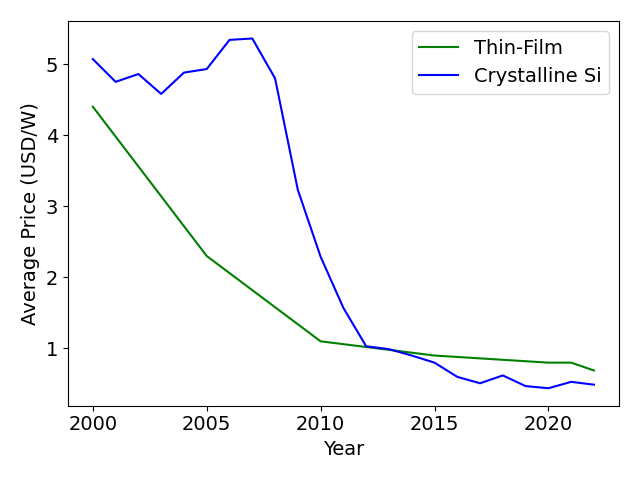
\includegraphics[width=0.5\linewidth]{Figures/Price Per Watt by Technology1.png}
    \caption{Price Per Watt by Technology over Time}
    \label{fig:enter-label}
\end{figure}

\begin{figure}
    \centering
    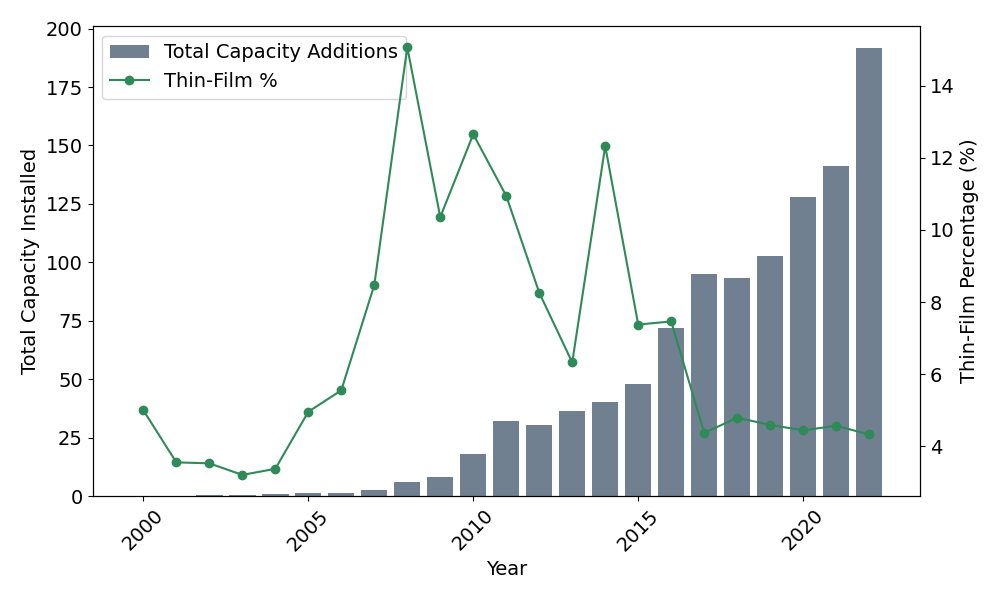
\includegraphics[width=0.5\linewidth]{Figures/ThinFilmPercentageAndCapacity.png}
    \caption{Total Capacity Installed and Thin Film Percentage}
    \label{fig:enter-label}
\end{figure}


\textcolor{blue}{insert two graphs:
\begin{enumerate}
    \item prices of major inputs for thin-film since 2000
    \item polysilicon price since 2000
\end{enumerate}
}

\begin{figure}
    \centering
    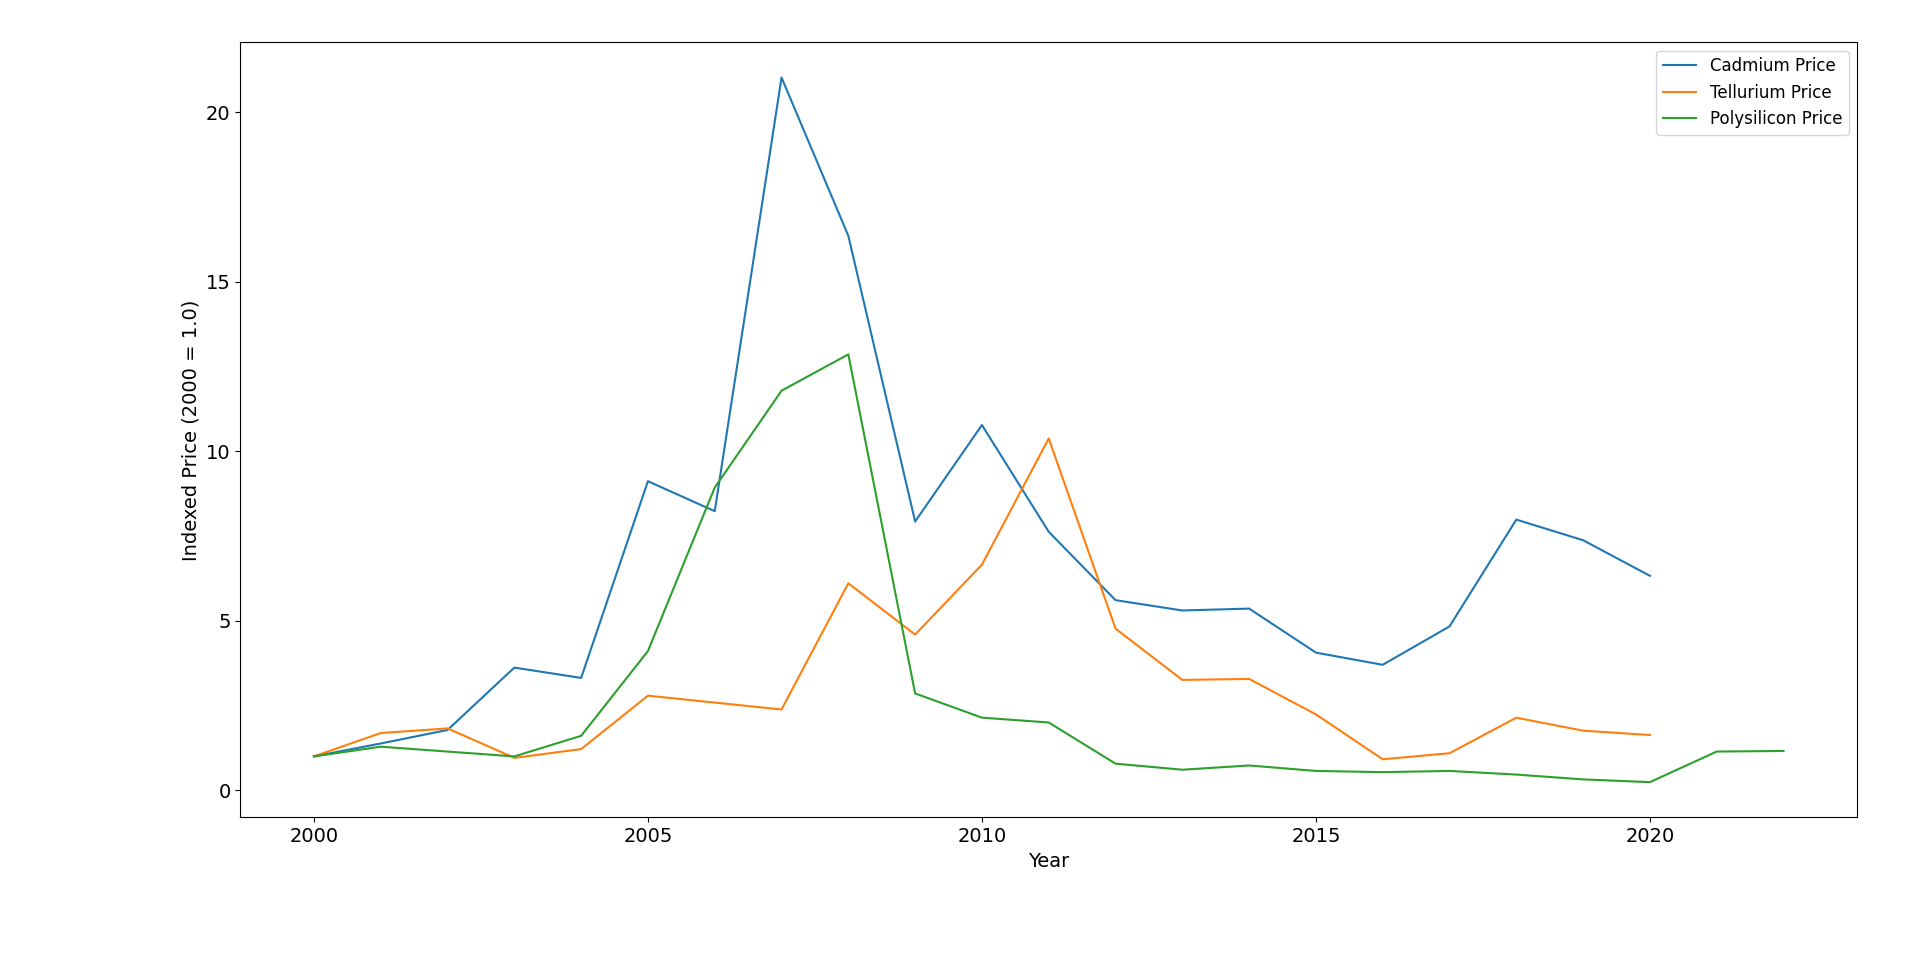
\includegraphics[width=0.5\linewidth]{Figures/Price by Material over Time.png}
    \caption{Price of Input Material by Material Type}
    \label{fig:enter-label}
\end{figure}


The polysilicon price spiked in late 2007. It encouraged investment in TFTs, which did not use the material. Meanwhile, it also induced massive investment in polysilicon production, which were concentrated in the U.S.. As new production came on line, along with the global recession staring in 2008, the polysilicon price receded quickly even lower than the presurge level. 

\textcolor{blue}{Graphs in Appendix:
\begin{enumerate}
    \item total production, share of poly-technology produced in each region (China, US, India, EU, Japan, ROW) since 2000
    \item total installation, share of poly-technology installed in each region (China, US, India, EU, Japan, ROW) since 2000
 %   \item price of each technology for each region (China, US, India, EU, Japan, ROW) since 2000
\end{enumerate}
}

\subsection{Polices around the World}
\label{subsec:inst_global_policy}

\begin{itemize}
    \item Policies on PV Installation:
        \begin{itemize}
        \item Tax rebates or credits that directly reduce the price that consumers need to pay. For example, \textcolor{red}{the US gave a direct subsidy of 30 percent of the system cost at the beginning of the period, which increased to 40 percent at the end of the period}.
        \item Feed-in tariff rate. \textcolor{red}{While the US preferred to promote adoption through tax subsidies, most of the rest of the world utilized feed-in-tariffs that encouraged production by solar producers. These feed-in-tariffs were non-trivial and got as high as 50 percent in Japan in 2012}.
        \item Tariffs on importing PV that increase the consumer price. \textcolor{red}{Over the period, tarriffs increased in response to dumping concerns with the greatest tariff increases coming in the United States to 35 percent at the end of the period and India at 20 percent at the end of the period.}
        \end{itemize}
    \item Policies on PV Manufacturing:
        \begin{itemize}
        \item Entry cost: low price/rent of land
        \item Marginal production cost: tax benefits
        \item Investment cost: low-interest loans
        \end{itemize}
\end{itemize}

\subsection{Chinese PV Manufacturing Industry}
\label{subsec:inst_china_PV}

China's PV manufacturing industry was miniscule in the early 2000s. 
The cell production was \textcolor{red}{XX} megawatts (MW) in 2000, accounting for less than 2 percent of the global supply. Production jumped to 14 percent in 2006 and grew fast in the next five years. It reached 60 percent by 2011 and has remained above that level since then.

%China’s PV manufacturing industry was miniscule before 2005.  It breached 100 megawatts (MW) of cell production in that year, jumping to 7 percent of global supply from less than 2 percent in 2003. Production grew by an order of magnitude in the next two years, another order of magnitude in the following three, and doubled again in 2011, capping roughly 200x growth in a six-year span. China’s share of the global market had surpassed 60 percent by 2011, and it has remained above that level since then.


\textcolor{blue}{insert graphs:
\begin{enumerate}
    \item China's output and number of firms by technology since 2000
    \item production shares of China, Japan, Germany, and US since 2000
    \item entry/exits of China, Non-China since 2000
    \item investment of each tech in China
\end{enumerate}
}



\begin{figure}
    \centering
    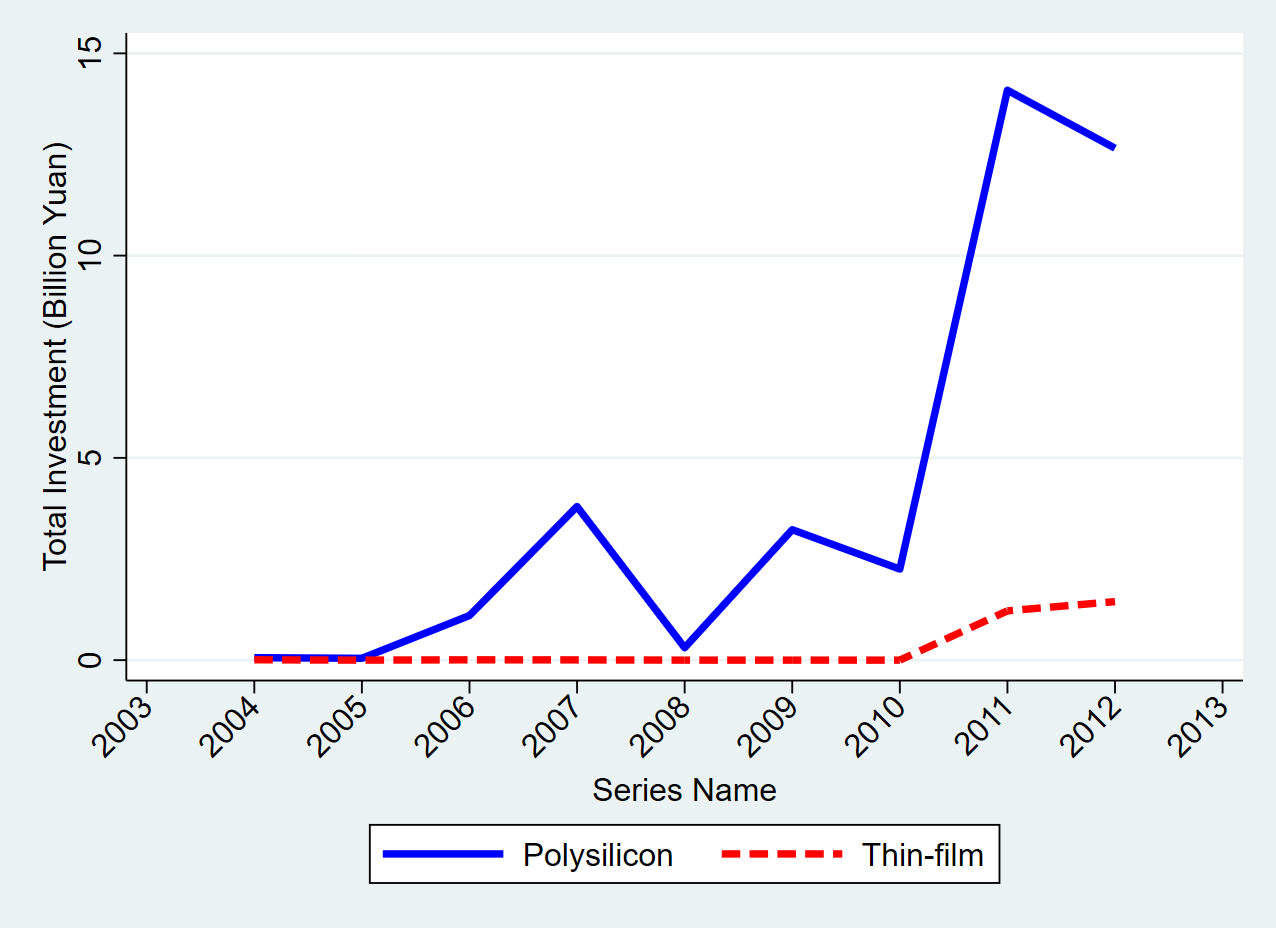
\includegraphics[width=0.5\linewidth]{Figures/InvestmentByFirmType.png}
    \caption{Investment by Firm-type}
    \label{fig:enter-label}
\end{figure}

\begin{itemize}
    \item China's subsidies on PV installation and Manufacturing:
        \begin{itemize}
        \item Entry cost: low price/rent of land
        \item Marginal production cost: tax benefits
        \item Investment cost: low-interest loans
        \item Demand: Golden Sun Project in China
        \end{itemize}
    \item Subsidies on polysilicon (input of the poly technology)
\end{itemize}

In the earlier phase of the surge, most of subsidies on PV production were provided by provincial and local government in the forms of low price or rent of land, low-interest loans, tax relief, and low electricity price.
%Provincial and local governments provide generous financial supports and tax reliefs to the production of solar PV. 
For example, Suntech in Jiangsu received an amount of \$3.7 billion low-interest loans from a state-owned bank and another \$1.4 billion in tax rebates and other export promotion subsidies between 2005 and 2012. \textcolor{red}{Cite source.} 

The central government intervened in the later phase of the surge. The State Council declared PV not just renewable energy in general but also a ``strategic emerging industry" in 2010. The state-owned banks fueled this industry with more than \$40 million of credits. \textcolor{red}{Cite source.} On the demand side, the central government introduced Golden Sun Project \textcolor{red}{that .... (more description).}

The central government also supported the creation of a domestic silicon industry, although the initial goal was to provide inputs for semiconductors rather than PV. \textcolor{red}{Cite source.} \textcolor{red}{China's production of polysilicon increased from xx in xx year to xxx in xx year. It was a major importer of polysilicon before XXX and can barely support its domestic needs since ... year.}

\subsection{Data}
\label{subsec:inst_data}

Our analysis combines data from various sources from 2000 to 2013. The first dataset contains quarterly information on the solar PV installation of each technology in six economic regions -- China, EU, India, Japan, US, and ROW.  \textcolor{red}{Data source.} 

The second data source is the annual database complied by the National Bureau of Statistics on Chinese manufacturing firms. For each PV manufacture and year, we observe its location (province), ownership status (state-owned, privately owned, or foreign firm), starting year of the firm.  We construct the capital stock and investment following the procedure by \citet{brandt2012creative} and \citet{barwick2025industrial}.


In addition, we obtain the quarterly global price per \textcolor{red}{Watt}  for each of the two technologies, quarterly global price for Polysilicon, Cadmium, and Tellurium. \textcolor{red}{Data on the quarterly price of Polysilicon comes from Bloomberg New Energy Finance and Bernreuter Research. Data on the price of Cadmium and Tellurium are taken from .} 
We also collect the information on demand policies in each region, including the tax credit or rebates, feed-in tariff rate, and importing tariff rate. \textcolor{red}{Tax credits and rebates and feed-in tariff rates are taken from .} 

Table \ref{tab:data_sum} reports the summary statistics on Chinese PV manufacturers.

\begin{table}[!h]
\centering
\caption{Summary Statistics on Chinese PV Manufacturers}
\label{tab:data_sum}
\begin{threeparttable}
\begin{tabularx}{0.7\textwidth}{Xcccccc}
\toprule
Variable & Mean & SD \\
\midrule
\multicolumn{3}{l}{\textit{Polysilicon PV:}} \\
%$\mathds{1}(\text{Polysilicon PV})$ &   &  \\
\quad Output (GW) &  .065 & .300 \\
\quad Investment &  9.32 & 32.90 \\
\quad Capital (Hundred Million Yuan) & 3.62  & 8.81 \\
\quad Age & 5.701  & 5.59 \\
\quad $\mathds{1}(\text{Private owned})$ & .435  & .496 \\
\quad $\mathds{1}(\text{Foreign JV})$ & .516 & .500 \\

\multicolumn{3}{l}{\textit{Thin-film PV:}} \\
%$\mathds{1}(\text{Polysilicon PV})$ &   &  \\
\quad Output (GW) & .024 & .070\\
\quad Investment (Million Yuan) & 9.59  & 17.1 \\
\quad Capital (Hundred Million Yuan) & 4.55  &6.63  \\
\quad Age &  5.67 & 4.48 \\
\quad $\mathds{1}(\text{Private owned})$ & .112  & .317 \\
\quad $\mathds{1}(\text{Foreign JV})$ & .806  &  .397 \\
\bottomrule
\end{tabularx}
\begin{tablenotes}
  \item  Notes: This table includes \textcolor{red}{912} firm-year level observations of polysilicon PV and \textcolor{red}{98} firm-year level observations of thin-film PV.
\end{tablenotes}
\end{threeparttable}
\end{table}

\section{Model}
\subsection{Model timing}

\begin{itemize}
    \item Notations: firm $j$, year $t$, technology $n$ ($n=1$ indexes thin-film and $n=2$ indexes polysilicon), economic region $m$ (US, EU, Japan, China, India, ROW)
\end{itemize}
Every year $t$,
    \begin{enumerate}
        \item Incumbent firms of technology $n$ observe production cost shock $\omega_{jnmt}$, choose quantity $q_{jnmt}$
        \item Incumbent firms of technology $n$ observe investment cost shock $\nu_{jnt}$, choose new investment $i_{jnt}$
        \item Incumbent firms of technology $n$ observe scrap value $\phi_{jnt}$, decide on exit. Entrants observe entry shock $\zeta_{jnt}$, decide whether to enter and if entering, which technology.
    \end{enumerate}

\subsection{Per-Period Demand and Production}

\subsubsection*{Demand}
The aggregate demand for technology-$n$ PV is given by:
\begin{equation}
Q_{nmt}=Q_{nm}(P_{1mt},P_{2mt},X_{mt}), \label{eq:model_demand}
\end{equation}
where $Q_{nmt}$ is the total units of technology-$n$ PV demanded by consumers in region $m$ in period $t$. $P_{nmt}$ is price of technology $n$ PV paid by consumers, which can be different from the global price $P_{nt}$ because of local tariffs and subsidies. In specific, the consumer-paying price
\[P_{nmt} = P_{nt}\times (1 + \text{tariff}_{mt}) - \text{subsidy}_{mt},\]
where $\text{tariff}_{mt}$ is the tariff rate that region $m$ collects in period $t$ and $\text{subsidy}_{mt}$ is the amount of demand subsidy that region $m$ grants.

$X_{mt}$ is a vector of demand shifters, such as aggregate indicators of the economic activity, region fixed effects, and year fixed effects.


\subsubsection*{Production}
The production cost of firm $j$ of technology $n$ that ships $q_{jnmt}$ units to region $m$ at time $t$ depends on the firm's output $q_{jnmt}$, a vector of state variables $s_{jnt}$, and a production shock $\omega_{jnmt}$:
    \begin{align}
         C^q_{nm}(q_{jnmt},s_{jnt},\omega_{jnmt}) \nonumber
    \end{align}
Here, $s_{jnt}$ includes firm characteristics (capital, age, location, ownership status), aggregate cost shifters affecting all firms (e.g. input price), policy dummies that capture the effect of industrial policies on production costs, such as indicators for specific time periods and indicators for specific provinces.

Firms compete in Cournot. They simultaneously choose how many units to produce for each region in each period, $q_{jnmt}$, taking as given other firms' production choice. If the equilibrium choice of $q_{jnmt}$ is positive, it satisfies the following first order condition:
 \begin{equation}
    P_{nmt}+q_{jnmt}^*\frac{\partial P_{nm}(Q_{nmt},X_{mt})}{\partial q_{jnmt}}=MC^q_{nm} (q_{jnmt}^*,s_{jnt},\omega_{jnmt}) \label{eq:model_foc_q}
\end{equation}   
where $MC^q_{nm} (q_{jnmt},s_{jnt},\omega_{jnmt})$ is the marginal product cost. 

Firm $j$'s expected profit before the production cost shocks are realized is given by:
\[
\pi_n(s_{jnt}) = \mathbb{E} [\sum_m \pi_{nm}(s_{jnt},\omega_{jnmt})]
\]
where $\pi_{nm}(s_{jnt},\omega_{jnmt})$ is firm $j$'s equilibrium profit from region $m$.

In each period, the global price of technology-$n$ products, $P_{nt}$, equates aggregate demand and supply, where the aggregate demand is given by equation (\ref{eq:model_demand}) and the aggregate supply is the sum of $q_{jnmt}^*$ defined in equation (\ref{eq:model_foc_q}).


\subsection{Incumbents: Investment and Exit}
At the end of each period, all incumbents observe a private scrap value that is drawn from a technology-specific distribution, and then decide whether to exit or remain active. We use $\phi_{jnt}$ to denote the scrap value of technology-$n$ incumbent $j$ and $F_{\phi,n}$ to denote the distribution. If a firm exits, it receives the scrap value. If it remains in operation, it observes an investment cost shock $\nu_{jnt}$ that is distributed i.i.d. with distribution $F_{\nu,n}$, and then choose the amount of investment $i_{jt}$ at cost $C_n^i(i_{jnt},s_{jnt},\nu_{jnt})$. This new investment is added to next period's capital stock which in turn affects its future production costs.

The value function of technology-$n$ incumbent $j$ after it observes the scrap value but without observing the realization of investment cost shock is:
\begin{eqnarray}
V_n(s_{jnt},\phi_{jnt})&=&\pi_n(s_{jnt})+\max\{\phi_{jnt},CV_n(s_{jnt})\}  \label{eq:incumbent_value_fn} 
\end{eqnarray}
where $CV_n(s_{jnt})$ is the continuation value, given by:
\begin{eqnarray}
CV_n(s_{jnt}) & \equiv & \mathbb{E}_{\nu}[-\{C_n^i(i^*,s_{jnt},\nu_{jnt})+\beta \mathbb{E}[V_n(s_{jnt+1})|s_{jnt},i^*]] \label{eq:incumbent_EV_fn}
\end{eqnarray}
where the expectation $\mathbb{E}_{\nu}$ is taken with respect to the investment cost shock $\nu_{jnt}$, and $i^* = i^*_n(s_{jnt},\nu_{jnt})$ is the optimal investment policy at state $s_{jnt}$ and investment cost shock $\nu_{jnt}$.
        
The optimal exit decision exhibits the threshold form. A firm exits if the scrap value exceeds the continuation value and remains active otherwise. Thus, the probability of exiting is given by:
\begin{eqnarray}
    p_n^x(s_{jnt}) & \equiv & Pr(\phi_{jnt} > CV_n(s_{jnt})) = 1-F_{\phi,n}(CV_n(s_{jnt})). \label{eq:exit_policy_fn}
\end{eqnarray}

Conditional on remaining active, technology-$n$ firm $j$'s optimal investment, $i^*=i_n^*(s_{jnt},\nu_{jnt})$, satisfies the following first order condition:
\begin{eqnarray}
    \beta\frac{\partial \mathbb{E}[V_n(s_{jnt+1})|s_{jnt},i]}{\partial i} &\leq & \frac{\partial C_n^i(i,s_{jnt},\nu_{jnt})}{\partial i} \label{eq:investment_policy_fn}
\end{eqnarray}

We assume that the marginal cost of investment has the following linear form:
\begin{eqnarray}
   MC_n^i(i_{jnt}, s_{jnt}, \nu_{jnt}) & = & s_{jnt} \rho^s_{n} + \rho^i_{n} i_{jnt} + \rho^{\nu}_{n} \nu_{jnt} \label{eq:investment_cost}
\end{eqnarray} 
where the investment cost shock $\nu_{jnt}$ is assumed to follow a standard normal distribution, independent of observed state variables $s_{jnt}$.

To capture the industrial policy that directly affect investment cost, we include policy dummies in $s_{jnt}$.


\textcolor{blue}{Note: Check whether incumbent firms divest during the period. If they do divest, we should include divestment in our analysis which would introduce a kink in the cost function and make the value function non-differentiable, raising considerable computational challenges. Check \citet{ryan2012costs} to see how to model both investment and divestment. }


\subsection{Potential Entrants: Entry and Technology}
In each period $t$, $\bar N$ potential entrants observe the profit shocks $\zeta_{j0t}$ if not entering, entry cost $\kappa_1(s_{jnt})-\zeta_{j1t}$ if entering with polysilicon technology, and $\kappa_2(s_{jnt})-\zeta_{j2t}$ if entering with thin film technology. $\kappa_1(s_{jnt})$ and $\kappa_2(s_{jnt})$ measure the expected entry costs of the two technology. Here $s_{jnt}$ include policy dummies to capture the effect of industrial policies on entry and technology choice.

After potential entrants observe their profit shocks $\zeta$'s, they decide on whether to enter and if entering, which technology. Thus, potential entrant $j$'s problem can be written as:
\begin{eqnarray}
 && max\{\zeta_{j0t}, max_{n\in \{1,2\}} \{-\kappa_n(s_{jnt}) + \zeta_{jnt} + VE_n(s_{jnt})\}\} \}
\end{eqnarray}
where $VE_n(s_{jnt})$ denotes the ex-ante value of entering with technology $n$ before observing investment cost shock:
\begin{eqnarray}
  VE_n(s_{jnt}) & \equiv & \mathbb{E}_{\nu}[-C_n^i(n_{jnt+1},s_{jnt},\nu_{jnt})+\beta \mathbb{E}[V_n(s_{jnt+1})|s_{jnt}]]\} \nonumber
\end{eqnarray}

A firm stays out of the market if its profit shock of not entering is higher than entering with either technology, enters with technology $n$ if that choice generates the highest profit. We use $p^{e,n}(s_{jnt})$ to denote the probability that potential entrant $j$ enters with technology $n$.
\begin{eqnarray}
  p^{e,n}(s_{jnt}) & \equiv & \text{Pr}\{\zeta_{jnt} - \zeta_{jn't}  > \kappa_n(s_{jnt})-\kappa_{n'}(s_{jn't}) + VE_{n'}(s_{jn't}) - VE_n(s_{jnt}) \nonumber \\
  & & \quad  \& \  \zeta_{jnt}-\zeta_{j0t} + >\kappa_n(s_{jnt})-VE_n(s_{jnt}) \} \label{eq:entry_policy_fn}
\end{eqnarray}



\subsection{Markov-Perfect Equilibrium}
A Markov-Perfect Equilibrium consists of policy function, $q_{jnmt},i^*_n(s_{jnt},\nu_{jnt}), p_n^x(s_{jnt}), p_n^e(s_{jnt})$, value function $V_n(s_{jnt})$, and global price $P_{nt}$, such that production quantity $q_{jnmt}^*$ satisfies (\ref{eq:model_foc_q}), investment policy function $i_n^*(s_{jnt},\nu_{jnt})$ satisfies (\ref{eq:investment_policy_fn}), exit policy function $p_n^x(s_{jnt})$ satisfies (\ref{eq:exit_policy_fn}), entry policy function $p_n^e(s_{jnt})$ satisfies (\ref{eq:entry_policy_fn}), global price $P_{nt}$ clears the market so that aggregate demand equals aggregate supply, and
incumbent's value function $V_n(s_{jnt})$ satisfies (\ref{eq:incumbent_value_fn}).

\subsection{Discussion of Model Assumptions}

Before moving on to the estimation, we discuss three key simplifications made by our model. First, we assume that solar PV are homogeneous conditional on production technology. \textcolor{blue}{Justifications. (i) homogeneous (citations) (ii) empirical evidence: price variation is small across producers conditional on geographic area and time.}

We assume that production is a static choice. One implication of this assumption is that we ignore learning-by-doing in the production. \citet{barwick2025drive} emphasizes the learning by doing in the EV battery production. In contrast, firms make dynamic decisions of investment that can potentially bring down the product cost in the future. \textcolor{blue}{More discussion. Complicated by allowing learning by doing in this framework?}

Lastly, we assume that government policies are perceived as permanent by all firms, as most studies in the literature such as \citet{ryan2012costs}. Relaxing this assumption requires \textcolor{blue}{...}, which would complicate our analysis substantially. See \citet{gowrisankaran2025policy} and \citet{chen2024dynamic} for more discussion.


\section{Estimation Strategy}
This section presents the estimation strategy to recover model parameters. The model contains five primitives: (i) the global demand function for solar PV of each technology, $Q_{jnmt}(\cdot)$, (ii) the production cost function for each technology, $C^q_{nm}(\cdot)$, (iii) the investment cost function for each technology, $C^i_{n}(\cdot)$, (iv) distribution of scrap value, and (v) the distribution of entry cost for each technology. Section \ref{subsec:est_static} describes the estimation of the static parameters, including those associated with the demand and production cost functions. Section \ref{subsec:est_dynamic} presents the two stage of estimation of the dynamic parameters, including parameters that are contained in the investment cost function and parameters that characterize the distributions of scrap value and entry cost. 



\subsection{Static Parameters: Demand and Production Cost}
\label{subsec:est_static}

\paragraph{Demand.} We parameterize the demand for solar PV of a technology in (\ref{eq:model_demand}) to be a simple Logit model. The demand of technology $n$ from region $m$ in year $t$ is given by:
\begin{eqnarray*}
Q_{nmt} & = & \frac{M_{mt}\cdot exp(-\alpha_{m} P_{nmt} + X_{mt}\eta +\xi_{nmt})}{1+\sum_{n'}exp(-\alpha_{m} P_{n'mt} + X_{mt}\eta +\xi_{n'mt})}  %\label{eq:demand_specification}
\end{eqnarray*}
where $M_{mt}$ is the market size of region $m$ in year $t$ (\textcolor{blue}{e.g., total electricity consumption}). $P_{nmt}$ is the price of technology $n$ that is faced by consumers in region $m$ which is the global price of that technology, $P_{nt}$, adjusted for local tariffs and subsidies. $X_{mt}$ is a vector of demand shifters, including electricity consumption, feed-in tariff, GDP, region FEs, and year FEs. 

Then, the empirical equation is
\begin{eqnarray}
ln( \frac{Q_{nmt}}{M_{mt}} ) - ln( \frac{M_{mt}- Q_{1mt}- Q_{2mt}}{M_{mt}} ) & = &  -\alpha_{m} P_{nmt} + X_{mt}\eta +\xi_{nmt}. \label{eq:demand_specification}
\end{eqnarray}
To deal with the price endogeneity, we use the price and production of major inputs. In specific, we instrument the price of polysilicon PV using the global price and production of polysilicon, and we instrument the price of thin film PV using the global prices and productions of cadmium and tellurium. The identification assumption is that input price and production are uncorrelated with the demand shocks for solar PV, $\epsilon_{nmt}$.  This is plausible for the following reasons. First, only a modest portion of global polysilicon production is used in solar PV production during this period, while the major demanders of polysilicon are the semiconductor manufacturing. \textcolor{red}{I am not sure we can make this argument. According to Bernreuter Research, 90 percent of polysilicon was used for solar panels at the end of the period. https://www.bernreuter.com/polysilicon/uses/.} Second, cadmium and tellurium are the by products of steel production, and the proportion of cadmium and tellurium is used in the thin-film PV production is negligible. \textcolor{red}{I'm also not sure we can make this argument. USGS considers thin-film solar as a major market for Cadmium https://www.usgs.gov/centers/national-minerals-information-center/cadmium-statistics-and-information. USGS also cites thin-film solar as the primary market for tellurium: https://pubs.usgs.gov/periodicals/mcs2024/mcs2024-tellurium.pdf} Lastly, the demand shock $\epsilon_{nmt}$ is at the region level. It is less of a concern that the demand shock for solar PV in a specific region is correlated with the global price of those major inputs.

\paragraph{Production Costs.} We parameterize the log of the marginal production cost for technology $n$ as a linear function:
    \begin{eqnarray}
       ln( MC^q_{nm} )&=&\gamma_{nm}^0+\gamma_{nm}^q q_{jnmt}+\gamma_n^s s_{jnt}+\omega_{jnmt} \label{eq:est_mc_q},
    \end{eqnarray}
where $q_{jnmt}$ denotes the units shipped by firm $j$ of technology $n$ to region $m$ in period $t$. $s_{jnt}$ is a vector of cost shifters. Firms' capital stock can potentially reduce their production cost, which motivates them to invest to accumulate capital. The prices of the major inputs also affect the production cost. In addition, the ownership status and whether it is a large firm are also included. As discussed in Section \ref{subsec:inst_china_PV}, the central government directly supported this industry between 2006 to 2008, and several provincial governments provide generous support. To capture these policy effects, we include a dummy between 2006 and 2008, a dummy for 2009 onwards, and indicators for Jiangsu and Zhejiang. $\omega_{jnmt}$ is the production cost shock.  %The production cost shock $\omega_{jnmt}$ is assumed to follow an i.i.d. normal distribution with mean zero and standard deviation of $\sigma_\omega$.

Under the specifications of Logit demand and linear marginal cost, the optimality condition of the Cournot competition implies
\begin{eqnarray}
  MC^q_{jnmt} &=&P_{nmt} - \frac{q_{jnmt}/Q_{nmt}}{\alpha_{m} \cdot (1-Q_{nmt}/M_{mt})}, \label{eq:est_foc_q}
\end{eqnarray}
where $q_{jnmt}/Q_{nmt}$ is the share of firm $j$'s sales among the total sales of that technology $n$ in the region-quarter ($mt$), and $Q_{nmt}/M_{mt}$ is the market share of technology $n$ in the region-quarter ($mt$).

We first obtain the implied marginal cost $\widehat{MC}^q_{jnmt}$ according to (\ref{eq:est_foc_q}). Then, we run the regression of the implied $log(\widehat{MC}^q_{jnmt})$ on its determinants specified in (\ref{eq:est_mc_q}) to obtain the parameters associated with the production cost, $\gamma \equiv (\gamma^0,\gamma^q,\gamma^s)$. One concern is that $q_{jnmt}$ can be negatively correlated with the marginal cost shock $\omega_{jnmt}$. To deal with this potential endogeneity issue, we use demand shifters as instrumental variables.


\begin{comment}
    \subsection{Static Parameters: Demand and Production Cost}
\label{subsec:est_static}

\paragraph{Demand.} We parameterize the demand for solar PV of a technology in (\ref{eq:model_demand}) to be a linear function of the price of that technology, the price of the competing technology, a vector of demand shifters, and a demand shock:
\begin{eqnarray}
  Q_{1mt} & = & \alpha^o_{1m} P_{1mt} + \alpha^c_{1m} P_{2mt}+X_{mt}\eta_{1m} +\epsilon_{1mt} \nonumber \\
  Q_{2mt} & = & \alpha^o_{2m} P_{2mt} + \alpha^c_{2m} P_{1mt}+X_{mt}\eta_{2m} +\epsilon_{2mt}, \label{eq:demand_specification}
\end{eqnarray}
where $Q_{nmt}$ is the total capacity of technology $n$ installed by region / quarter. $P_{nmt}$ is the price of technolgy $n$ that is faced by consumers in region $m$ which is the global price of that technology, $P_{nt}$, adjusted for local tariffs and subsidies. $X_{mt}$ is a vector of demand shifters, including electricity consumption, feed-in tariff, GDP, region FEs, and year FEs. $\alpha^o_{nm}$ captures the own price effect, and $\alpha^c_{nm}$ captures the cross price effect.

To deal with the price endogeneity, we use the price and production of major inputs. In specific, we instrument the price of polysilicon PV using the global price and production of polysilicon, and we instrument the price of thin film PV using the global prices and productions of cadmium and tellurium. The identification assumption is that input price and production are uncorrelated with the demand shocks for solar PV, $\epsilon_{nmt}$.  This is plausible for the following reasons. First, only a modest portion of global polysilicon production is used in solar PV production during this period, while the major demanders of polysilicon are the semiconductor manufacturing. \textcolor{red}{I am not sure we can make this argument. According to Bernreuter Research, 90 percent of polysilicon was used for solar panels at the end of the period. https://www.bernreuter.com/polysilicon/uses/.} Second, cadmium and tellurium are the by products of steel production, and the proportion of cadmium and tellurium is used in the thin-film PV production is negligible. \textcolor{red}{I'm also not sure we can make this argument. USGS considers thin-film solar as a major market for Cadmium https://www.usgs.gov/centers/national-minerals-information-center/cadmium-statistics-and-information. USGS also cites thin-film solar as the primary market for tellurium: https://pubs.usgs.gov/periodicals/mcs2024/mcs2024-tellurium.pdf} Lastly, the demand shock $\epsilon_{nmt}$ is at the region level. It is less of a concern that the demand shock for solar PV in a specific region is correlated with the global price of those major inputs.

\paragraph{Production Costs.} We parameterize the marginal product cost for technology $n$ as a linear function:
    \begin{equation}
        MC_{nm}(q_{jnmt},s_{jnt},\omega_{jnmt})=\gamma_{nm}^0+\gamma_{nm}^q q_{jnmt}+\gamma_n^s s_{jnt}+\omega_{jnmt}  \nonumber
    \end{equation}
where $q_{jnmt}$ denotes the units shipped by firm $j$ of technology $n$ to region $m$ in period $t$. $s_{jnt}$ is a vector of cost shifters. Firms' capital stock can potentially reduce their production cost, which motivates them to invest to accumulate capital. The prices of the major inputs also affect the production cost. In addition, the ownership status and whether it is a large firm are also included. As discussed in Section \ref{subsec:inst_china_PV}, the central government directly supported this industry between 2006 to 2008, and several provincial governments provide generous support. To capture these policy effects, we include a dummy between 2006 and 2008, a dummy for 2009 onwards, and indicators for Jiangsu and Zhejiang. The production cost shock $\omega_{jnmt}$ is assumed to follow an i.i.d. normal distribution with mean zero and standard deviation of $\sigma_\omega$.

Under the specifications of linear demand and linear marginal cost, the optimality condition of the Cournot competition is
\begin{eqnarray*}
  q_{jnmt}^*&=&\frac{P_{nmt}-\gamma_{nm}^0-s_{jnt}\gamma_n^s-\omega_{jnmt}}{\gamma_{nm}^q-\alpha_{nm}}  \\
  q_{jnmt}&=&max(0,q_{jnmt}^*)
\end{eqnarray*}

Let $\gamma$ summarize all parameters associated with the  production cost, $\gamma = (\gamma^0,\gamma^q,\gamma^s,\sigma_\omega)$. We estimate these parameters using a Tobit Model:
\begin{eqnarray*}
    L(\gamma)&=&\prod_{j,n,m,t;q_{jnmt}=0} Pr(q_{jnmt}=0|s_{jnt};\gamma_n)\times\prod_{j,n,m,t;q_{jnmt}>0} f_{q,n}(q_{jnmt}|s_{jnt};\gamma_n)
\end{eqnarray*}

\textcolor{blue}{Note: Check the proportion of $q_{jnmt}$ that have zero values. If this proportion is very small, we can ignore this event and don't need to use Tobit model. Instead, we can use Logit demand and invert the FOC to get the MC. Then run a regression of the implied MC on $s_{jnt}$ and $q_{jnmt}$ using appropriate IVs.}
\end{comment}

\subsection{Dynamic Parameters}
\label{subsec:est_dynamic}
Dynamic parameters are estimated using the observed decisions of firm investment, exit, and entry (not enter, enter with polysilicon technology, or enter with thin-film technology). Following the BBL approach of \citet{bajari2007estimating}, we estimate the parameters in two stages. In the first stage, we flexibly estimate policy functions, including investment, exit, and entry, as well as the transition process of state variables from the data directly. After that, we flexibly approximate the value function by a set of B-spline basis functions of state variables (\citet{sweeting2013dynamic}). In the second stage, we estimate the dynamic parameters using maximum likelihood estimation approach. Additional details are relegated to the Appendix \textcolor{red}{XX}.


\subsubsection{First Stage}
\paragraph{Exit Policy Function} 
We assume that the scrap value follows a normal distribution. Then, we can run a Probit regression as follows
\begin{equation}
    Pr_n(\chi_{jnt}=1|s_{jnt})=\Phi(h_n(s_{jnt})),
\end{equation}
where $\chi_{jnt}=1$ if firm $j$ of technology $n$ exits in period $t$, $h_n(s_{jnt})$ is a technology-specific polynomial function of the states, and $\Phi$ is the cdf of standard normal distribution. We use $\hat{p}^x_n(s)$ to denote the estimated exit probability at state $s$.



\paragraph{Investment Policy Function}
As shown in \citet{bajari2007estimating}, the optimal investment policy function $i_n^*(s_{jnt},\nu_{jnt})$ is monotonically decreasing in the shock $\nu_{jnt}$ and can be recovered as follows:
\begin{eqnarray}
i_n^*|s_{jnt} &=& G^{-1}(1-F_{\nu,n}(\nu\mid s_{jnt})) \label{eq:est_investment}
\end{eqnarray}
where $G(i\mid s_{jnt})$ is the empirical distribution of investment given the state variables, and $F_{\nu,n}(\nu\mid s_{jnt})$ is the assumed distribution of $\nu$.

We can rewrite the optimal investment as the sum of two components, with one being a function of the state variables and the other one being a function of the shock:
\begin{eqnarray}
i_{jnt}^* &=& h_{1n}(s_{jnt})+h_{2n}(\nu_{jnt}),
\end{eqnarray}
where $h_{1n}(\cdot)$ and $h_{2n}(\cdot)$ are two unknown functions to be estimated.

We first flexibly regress $i_{jnt}$ on $s_{jnt}$ non-parametrically to get the estimate $\hat{h}_{1n}(s_{jt})$ and hence $i^*_{jnt}-\hat{h}_{1n}(s_{jt})$. Then, we estimate $h_{2n}(\cdot)$ using (\ref{eq:est_investment}).


\paragraph{State Transition}
The state variable $s_{jnt}$ includes the state of all firms in the industry and hence is high-dimensional. To reduce the dimension, we assume that firms do not keep track of the state variables of every rival and use industry-level prices as a sufficient statistic, similar to the oblivious equilibrium concept  (\citet{weintraub2008markov} and \citet{benkard2015oblivious}). This is a reasonable assumption given that the industrial HHI is \textcolor{blue}{XXX} and market power is not a big concern. A similar assumption has often been adopted in the literature, for example, \citet{jeon2022learning}, \citet{chen2023structural}, and \citet{barwick2025industrial}.

Furthermore, notice that the state variables enter the marginal production cost linearly in our model. It suggests that what really matters is the one-dimensional index $\bar s_{jnt} = -s_{jnt} \hat \gamma_n^s$, named cost efficiency. Hence, we assume that firms keep track of the index $\bar s_{jnt}$ instead of each element of the vector $s_{jnt}$.

Some of the state variables, such as firm location, ownership status, are fixed over time. The firm age transits deterministically. As for capital stock, we assume that it depreciates at a common rate $\delta$ with a quarterly value of 2.3\%:
\[
k_{jnt+1}  = (1-\delta) k_{jnt} + i_{jnt}.
\]

The equilibrium price for each PV type clears the market by equalizing the aggregate demand and aggregate supply and hence is a complicated object. Following \citet{barwick2025industrial} and other work, we model it as an AR(1) process. We allow that different technologies to have different price processes. In addition, for polysilicon PV, we allow the process to differ before 2007 and after 2011.
(\textcolor{blue}{What we do as for the PV price during 2008-2011 when the price drops substantially?)}

We make similar assumptions for the input prices. For each input, we specify different processes before the spike and after spike. (\textcolor{blue}{Note: The three inputs have different spike time.})


\paragraph*{Value Function Approximation}
We assume the scrap value $\phi_{jnt}$ follows an exponential distribution with parameter $1/\sigma_{\phi}$. \textcolor{blue}{(Note: we can allow the parameter to differ across the two technologies, $1/\sigma_{\phi,n}$)}. The ex-ante value function, before the realization of $\phi_{jnt}$, is
\begin{eqnarray}
    V_n(s_{jnt}) & = & \mathbb{E}_\phi[\pi_n(s_{jnt}) + max\{\phi_{jnt},CV_n(s_{jnt})\}] \nonumber \\
    & = & \pi(s_{jnt}) + p_n^x(s_{jnt}) \sigma_\phi + CV_n(s_{jnt})
\end{eqnarray}
where $\pi(s_{jnt})$ denotes firms' static profit, $p_n^x(s_{jnt})$ denote their exit probability, and $CV_n(s_{jnt})$ denote their continuation value defined in (\ref{eq:incumbent_EV_fn}).

Following the literature (e.g., \citet{sweeting2013dynamic}), we approximate the ex-ante value function using B-spline basis functions of the state variables. That is, $V_n(s_{jnt}) = \sum_l \lambda_{n,l} u_{n,l}(s_{jnt})$ where $u_{n,l}(s_{jnt})$ are basis functions and $\lambda_{n,l}$ are coefficients to be estimated.


\subsubsection{Second Stage: MLE}
\paragraph{Scrap Value and Investment Costs}
The dynamic parameters are summarized in $\theta = (\sigma_\phi, \rho^s_n, \rho^i_n, \rho^{\nu}_n )$. We allow the constant term in the marginal investment cost, $\rho^s_n$, to differ before and after the policy period and differ across provinces, to capture the central and local government subsidies on investment. 


Let $\chi_{jnt}$ indicate firm $j$ of technology $n$ exits in year $t$ in the data. Then, the log-likelihood of its exiting decision is
\begin{eqnarray}
    log(f_{n}(\chi_{jnt};\theta)) &=& \Big[ (1-\chi_{jnt}) log(1-exp(-\frac{CV_n(s_{jnt};\theta)}{\sigma_\phi})) - \chi_{jnt} \frac{CV_n(s_{jnt};\theta)}{\sigma_\phi} \Big].
\end{eqnarray}

The likelihood of positive investment is
\begin{eqnarray}
    g_n(i_{jnt};\theta) &=& \frac{f_\nu(\nu_{jnt})}{|\partial i_n^*(s_{jnt},\nu_{jnt}) /\partial \nu_{jnt}|},
\end{eqnarray}
and the likelihood of non-positive investment is
\begin{eqnarray}
    g_n(i_{jnt};\theta) &=& Pr\Big( [\beta\frac{\partial \mathbb{E}[V_n(s_{jnt+1})|s_{jnt},i]}{\partial i} - \frac{\partial C_n^i(i,s_{jnt},\nu_{jnt})}{\partial i}]_{i=0} \leq 0  \Big).
\end{eqnarray}

The maximum likelihood estimate maximizes the joint log-likelihood of exiting and investment.   
\begin{eqnarray}
        max_\theta L(\theta) & = & \sum_{j,n,t} log(f_n(\chi_{jnt};\theta)) + \sum_{j,n,t} log(g_n(i_{jnt};\theta)) \nonumber \\
        s.t. \ V_n(s_{jnt};\theta) & = & \pi_n(s_{jnt}) + p_n^x(s_{jnt}) \sigma_\phi + CV_n(s_{jt};\theta)  \nonumber
\end{eqnarray}
where $f_n(\chi_{jnt};\theta)$: Prob. of exit
$g_n(i_{jnt};\theta)$: Density of investment


\paragraph{Entry Costs}
We further assume that the profit shocks $\zeta$ follows the i.i.d. T1EV distributional. Then, the probability that potential entrant $j$ enters with technology $n$ is
\begin{eqnarray*}
  p^{e,n}(s_{jnt}) & \equiv & \frac{exp\Big(-\kappa_n(s_{jnt}) + VE_n(s_{jnt}) \Big)}{1 + exp\Big(-\kappa_1(s_{jnt}) + VE_1(s_{j1t})\Big) + exp\Big(-\kappa_2(s_{jnt}) + VE_2(s_{j2t})\Big)}. %\label{eq:entry_policy_fn}
\end{eqnarray*}
Then, we estimate the mean entry costs using the observed entry decisions via MLE.


\section{Estimation Results}


\subsection{Static Parameters}

\subsubsection{Demand}

Table \ref{tab:est_demand} reports the estimates of parameters in the demand equation, where column (1) has the same price coefficient and column (2) allows the price coefficients to differ across regions. 

\textcolor{blue}{We can play by including or excluding GDP, region FE, year FE. We can also play by allowing or not allowing the price coefficients to be regional specific. We can also try different market size measures.}

Expected results:
\begin{itemize}
    \item price coefficient to be negative
    \item variations in price coefficients across regions. US, Japan, Germany have smaller price sensitivity 
    \item coefficient before the indicator of polysilicon-PV to be positive
    \item coefficient before electricity consumption to be positive
    \item coefficient before feed-in tariff rate to be positive
\end{itemize}


\begin{table}[!h]
\centering
\caption{Demand Estimates}
\label{tab:est_demand}
\begin{threeparttable}
\begin{tabularx}{1.00\textwidth}{Xlllllll}
\toprule
 & \multicolumn{2}{c}{(1)}  && \multicolumn{2}{c}{(3)} \\
\cmidrule{2-3} \cmidrule{5-6}
 & Est. & SE   && Est. & SE \\
\midrule
\multicolumn{6}{l}{PV price ($\alpha_m$)} \\
\quad $\times$ China & -1.168\sym{***} & (0.111) && -1.428\sym{***} & (0.122) \\
\quad $\times$ EU     & -0.997\sym{***} & (0.105) && -1.116\sym{***} & (0.107) \\
\quad $\times$ India  & -1.317\sym{***} & (0.116) && -1.243\sym{***} & (0.130) \\
\quad $\times$ Japan  & -0.720\sym{***} & (0.090) && -0.779\sym{***} & (0.093) \\
\quad $\times$ US     & -1.142\sym{***} & (0.113) && -1.206\sym{***} & (0.125) \\
\quad $\times$ ROW    & -1.204\sym{***} & (0.101) && -1.469\sym{***} & (0.095) \\[0.3em]

\multicolumn{6}{l}{Demand shifters ($\eta$)} \\
\quad \mathds{1}(Poly-PV) & 3.214\sym{***} & (0.360) && & \\
\quad\quad $\times$ China & & && 3.654\sym{***} & (0.383) \\
\quad\quad $\times$ EU & & && 3.983\sym{***} & (0.338) \\
\quad\quad $\times$ India & &  && 2.641\sym{***} & (0.402) \\
\quad\quad $\times$ Japan & &  && 3.526\sym{***} & (0.331) \\
\quad\quad $\times$ US & & && 2.388\sym{***} & (0.359) \\
\quad\quad $\times$ ROW & & && 3.599\sym{***} & (0.356) \\
\quad GDP & 9.49\sym{***} & (1.72) && 2.41\sym{*} & (1.34) \\
\quad Feed-in tariff & 1.954\sym{***} & (0.531) && 1.898\sym{***} & (0.573) \\
\quad Constant & -30.422\sym{***} & (0.366)  && -29.411\sym{***} & (0.250) \\

\midrule
\(R^2\)                      & \multicolumn{2}{c}{0.731} &&  \multicolumn{2}{c}{0.809} \\
\bottomrule
\end{tabularx}
\begin{tablenotes}
\footnotesize
\item Notes: 239 observations in each regression. Standard errors in parentheses.
\sym{*}\,$p<0.10$, \sym{**}\,$p<0.05$, \sym{***}\,$p<0.01$.
\end{tablenotes}
\end{threeparttable}
\end{table}
\subsubsection{Production Cost}

Table \ref{tab:est_marginal_cost} reports the estimation results of the marginal cost functions of polysilicon firms and thin film firms, separately.

Expected results:
\begin{itemize}
    \item $\beta^q$ can be either positive (diseconomy of scale) or negative (economy of scale)
    \item Coefficients before 2006-2008 and post-2008 are expected to be negative. These capture the subsidy on production cost during these periods.
    \item Coefficients before Jiangsu, Zhejiang, Anhui are expected to be negative, capturing local subsidy on production costs in these provinces.
\end{itemize}

\textcolor{blue}{We can play by allowing or not allowing $\gamma^0_{nm}$ to vary across regions, $\gamma^0_{nm}$ to be different across technology. We can play the same thing for $\gamma^q_{nm}$. We can also play by including or excluding some state variables, not allowing some to be technology specific.}

% \begin{table}[!h]
% \centering
% \caption{Marginal Production Cost Equation}
% \label{tab:iv_est_marginal_cost_rescaled}
% \begin{threeparttable}
% \begin{tabularx}{0.92\textwidth}{Xllllll}
% \toprule
%  & \multicolumn{2}{c}{Polysilicon PV (IV)} && \multicolumn{2}{c}{Thin-Film PV (IV)} \\
% \cmidrule{2-3} \cmidrule{5-6}
%  & Est. & SE && Est. & SE \\
% \midrule
% \multicolumn{5}{l}{\textit{Constant ($\gamma^0_{nm}$)}}\\
% \quad Constant & 29.95\sym{***} & (1.72) && & \\
% \quad $\times$ ROW  & 1.23 & (1.70) && & \\
% \quad $\times$ EU   & 2.23 & (1.72) && & \\
% \quad $\times$ Japan & 1.40 & (1.80) && & \\
% \quad $\times$ India & 1.48 & (1.87) && & \\
% \quad $\times$ US    & $-3.05$\sym{*} & (1.77) && & \\[0.4em]

% \multicolumn{5}{l}{\textit{Output ($\gamma^q$)}}\\
% \quad Quantity (IV) & 9.51 & (6.40) && & \\[0.6em]

% \multicolumn{5}{l}{\textit{Technology-specific state variables ($\gamma^s_n$)}}\\
% \quad Cadmium price && && $-1.11$ & (3.65) \\
% \quad Tellurium price && && 6.34 & (4.04) \\
% \quad Polysilicon price & 3.58\sym{***} & (0.40) && & \\
% \quad Jiangsu × Post-2008 & 0.54 & (0.42) && 1.39 & (1.34) \\
% \quad Zhejiang × Post-2008 & $-0.037$ & (0.44) && 1.33 & (1.25) \\

% \multicolumn{5}{l}{\textit{Common state variables ($\gamma^s$)}}\\
% \quad Capital & $-2.49$\sym{***} & (0.43) && & \\
% \quad Capital$^2$ & 3.47\sym{***} & (0.65) && & \\
% \quad Learning by Doing & $-8.95$\sym{***} & (0.199) && & \\[0.4em]
% \quad Post-2008 & $-18.41$\sym{***} & (.636) && & \\[0.4em]
% \quad Age & $-0.58$\sym{***} & (0.03) && & \\
% \quad Foreign JV & 0.72 & (0.56) && & \\
% \quad Private & 0.07 & (0.58) && & \\
% \quad Large firm & 2.31\sym{***} & (0.49) && & \\

% \midrule
% Region FE                    & \multicolumn{2}{c}{Y} && \multicolumn{2}{c}{Y} \\
% $N$ & \multicolumn{2}{c}{1,811} && \multicolumn{2}{c}{112} \\
% \bottomrule
% \end{tabularx}

% \begin{tablenotes}\footnotesize
% \item Notes: G2SLS random-effects IV estimates of marginal-cost functions. Quantity is instrumented using real GDP and feed-in tariff policy by technology. Standard errors in parentheses.
% \item \sym{*}\,$p<0.10$, \sym{**}\,$p<0.05$, \sym{***}\,$p<0.01$.
% \end{tablenotes}
% \end{threeparttable}
% \end{table}

\begin{table}[!h]
\centering
\caption{Marginal Production Cost Equation}
\label{tab:iv_est_marginal_cost_rescaled}
\begin{threeparttable}
\begin{tabularx}{0.92\textwidth}{Xllllll}
\toprule
 & \multicolumn{2}{c}{Polysilicon PV (IV)} && \multicolumn{2}{c}{Thin-Film PV (IV)} \\
\cmidrule{2-3} \cmidrule{5-6}
 & Est. & SE && Est. & SE \\
\midrule
\multicolumn{5}{l}{\textit{Constant ($\gamma^0_{nm}$)}}\\
\quad Constant & 10.06\sym{***} & (2.68) && & \\
\quad $\times$ ROW  & 5.47\sym{*} & (3.31) && & \\
\quad $\times$ EU   & 6.58\sym{**} & (3.34) && & \\
\quad $\times$ Japan & 6.26\sym{*} & (3.50) && & \\
\quad $\times$ India & 5.93 & (3.67) && & \\
\quad $\times$ US    & 1.02 & (3.46) && & \\[0.4em]

\multicolumn{5}{l}{\textit{Output ($\gamma^q$)}}\\
\quad Quantity (IV) & 27.56\sym{***} & (9.15) && & \\[0.6em]

\multicolumn{5}{l}{\textit{Technology-specific state variables ($\gamma^s_n$)}}\\
\quad Cadmium price && && 0.00081 & (0.00054) \\
\quad Tellurium price && && $-3.95$ & (5.98) \\
\quad Polysilicon price & 0.0120\sym{***} & (0.00035) && & \\
\quad Jiangsu × Post-2008 & $-2.37$\sym{***} & (0.62) && 0.40 & (2.00) \\
\quad Zhejiang × Post-2008 & $-2.97$\sym{***} & (0.66) && 1.05 & (1.87) \\

\multicolumn{5}{l}{\textit{Common state variables ($\gamma^s$)}}\\
\quad Capital & $-4.57$\sym{***} & (0.66) && & \\
\quad Capital$^2$ & $5.24$\sym{***} & (1.09) && & \\
\quad Learning by Doing & $-1.20$\sym{***} & (.286) && & \\[0.4em]
\quad Age & $-0.81$\sym{***} & (0.05) && & \\
\quad Foreign JV & 0.69 & (0.86) && & \\
\quad Private & 0.60 & (0.88) && & \\
\quad Large firm & 4.82\sym{***} & (0.71) && & \\

\midrule
Region FE                    & \multicolumn{2}{c}{Y} && \multicolumn{2}{c}{Y} \\
$N$ & \multicolumn{2}{c}{1,811} && \multicolumn{2}{c}{112} \\
\bottomrule
\end{tabularx}

\begin{tablenotes}\footnotesize
\item Notes: G2SLS random-effects IV estimates of marginal-cost functions. Quantity is instrumented using real GDP and feed-in tariff policy by technology. Standard errors in parentheses.
\item \sym{*}\,$p<0.10$, \sym{**}\,$p<0.05$, \sym{***}\,$p<0.01$.
\end{tablenotes}
\end{threeparttable}
\end{table}
\begin{comment}
    \subsection{Static Parameters}

\subsubsection{Demand}

Table \ref{tab:reg_demand_china} reports the estimates of parameters in the demand equation, where column (1) reports the estimates for polysilicon and column (2) reports the estimates for thin-film. Column (3) and (4) allow the price coefficients to differ across regions. 

\textcolor{blue}{We can play by including or excluding GDP, region FE, year FE. We can also play by allowing or not allowing the price coefficients to be regional specific.}

Expected results:
\begin{itemize}
    \item own-price coefficient to be negative, cross-price coefficient to be positive
    \item magnitude of own-price coefficient is larger than that of cross-price coefficient
    \item Polysilicon PV has a smaller price sensitivity than thin-film PV
    \item variations in price coefficients across regions. US, Japan, Germany have smaller price sensitivity 
    \item coefficient before electricity consumption to be positive
    \item coefficient before feed-in tariff rate to be positive
\end{itemize}


\begin{table}[!h]
\centering
\caption{Estimates of Demand Parameters}
\label{tab:reg_demand_china}
\begin{threeparttable}
\begin{tabularx}{0.92\textwidth}{Xcccccc}
\toprule
 & \multicolumn{2}{c}{Polysilicon PV} && \multicolumn{2}{c}{Thin-Film PV} \\
\cmidrule{2-3} \cmidrule{5-6}
 & Est. & SE && Est. & SE \\
\midrule
\multicolumn{5}{l}{Price of polysilicon PV} \\
\quad $\times$ China & $-4.572$\sym{**} & $(2.018)$ && $-0.147$ & $(0.153)$ \\
\quad $\times$ EU    & $-7.920$\sym{***}& $(2.370)$ && $-0.293$ & $(0.179)$ \\
\quad $\times$ India & $-2.325$\sym{*}  & $(1.318)$ && $-0.181$\sym{*} & $(0.100)$ \\
\quad $\times$ Japan & $-5.336$\sym{**} & $(2.215)$ && $-0.034$ & $(0.168)$ \\
\quad $\times$ US    & $-8.547$\sym{***}& $(2.692)$ && $-0.642$\sym{***}& $(0.204)$ \\
\quad $\times$ ROW   & $-5.014$\sym{***}& $(1.288)$ && $-0.217$\sym{**} & $(0.098)$ \\[0.3em]

\multicolumn{5}{l}{Price of thin-film PV } \\
\quad $\times$ China & $ 5.960$ & $(4.480)$ && $-0.150$ & $(0.339)$ \\
\quad $\times$ EU    & $ 4.010$ & $(3.370)$ && $-0.113$ & $(0.255)$ \\
\quad $\times$ India & $ 1.370$ & $(2.410)$ && $ 0.091$ & $(0.182)$ \\
\quad $\times$ Japan & $ 6.390$ & $(3.890)$ && $-0.069$ & $(0.294)$ \\
\quad $\times$ US    & $ 5.890$\sym{*} & $(3.060)$ && $ 0.354$ & $(0.232)$ \\
\quad $\times$ ROW   & $-0.510$ & $(2.400)$ && $-0.056$ & $(0.182)$ \\[0.3em]

Electricity consumption      & $  8.881$\sym{*} & $(4.542)$ && $-0.172$ & $(0.344)$ \\
Feed-in tariff rate          & $ 22.058$\sym{**}& $(9.940)$ && $ 1.573$\sym{**}& $(0.752)$ \\
Constant                     & $ -8.738$        & $(25.638)$&& $ 1.468$ & $(1.941)$ \\
\midrule
Region FE                    & \multicolumn{2}{c}{Y} && \multicolumn{2}{c}{Y}\\
Year FE                      & \multicolumn{2}{c}{Y} && \multicolumn{2}{c}{Y}\\
\(R^{2}\)                    & \multicolumn{2}{c}{0.770} && \multicolumn{2}{c}{0.653}\\
\bottomrule
\end{tabularx}
\begin{tablenotes}
\footnotesize
\item Notes: 126 observations in each specification.  Standard errors in parentheses.
      \sym{*}\,$p<0.10$, \sym{**}\,$p<0.05$, \sym{***}\,$p<0.01$.
      All regressions include region and year fixed effects (not reported).
      Prices of polysilicon PV and thin-film PV are instrumented with global polysilicon,
      cadmium, and tellurium prices, respectively.
\end{tablenotes}
\end{threeparttable}
\end{table}

\subsubsection{Production Cost}

Table \ref{tab:est_marginal_cost} reports the estimation results of the marginal cost functions of polysilicon firms and thin film firms, separately.

Expected results:
\begin{itemize}
    \item $\beta^q$ can be either positive (diseconomy of scale) or negative (economy of scale)
    \item Coefficients before 2006-2008 and post-2008 are expected to be negative. These capture the subsidy on production cost during these periods.
    \item Coefficients before Jiangsu, Zhejiang, Anhui are expected to be negative, capturing local subsidy on production costs in these provinces.
\end{itemize}

\textcolor{blue}{We can play by allowing or not allowing $\gamma^0_{nm}$ to vary across regions, $\gamma^0_{nm}$ to be different across technology. We can play the same thing for $\gamma^q_{nm}$. We can also play by including or excluding some state variables, not allowing some to be technology specific.}

\begin{table}[!h]
\centering
\caption{Estimates of Marginal-Cost Functions}
\label{tab:est_marginal_cost}
\begin{threeparttable}
\begin{tabularx}{0.92\textwidth}{Xcccccc}
\toprule
 & \multicolumn{2}{c}{Polysilicon PV} && \multicolumn{2}{c}{Thin-Film PV} \\
\cmidrule{2-3}\cmidrule{5-6}
 & Est. & SE && Est. & SE \\
\midrule
\multicolumn{5}{l}{\textit{Constant ($\gamma^{0}_{nm}$)}}\\
\quad Constant                               &   28.362\sym{***} & (0.940) &&  4.041 & (2.500) \\[0.4em]

\multicolumn{5}{l}{\textit{Output ($\gamma^{q}$)}}\\
                                             & -0.576 & (0.724) &&  1.336 & (6.833) \\[0.6em]

\multicolumn{5}{l}{\textit{Technology-specific state variables ($\gamma^{s}_{n}$)}}\\
\quad Polysilicon price             & 11.087\sym{***} & (0.987) &&        &        \\
\quad Cadmium price&&               &&  2.038\sym{***} & (0.655) \\
\quad Tellurium price &&            && -3.610         & (5.840) \\
\quad Capital            & -2.360\sym{***} & (0.363) && -3.720 & (3.300) \\
\quad Capital$^{2}$ &  0.274\sym{***} & (0.068) &&  1.120 & (0.835) \\

\multicolumn{5}{l}{\textit{Common state variables ($\gamma^{s}_{n}$)}}\\
\quad 2006--2008                              &     -16.145\sym{***}& (1.293) &&        &        \\
\quad Post-2008                               & -18.849\sym{***}& (0.559) &&        &        \\
\quad Jiangsu                                  & -0.149         & (0.472) &&        &        \\
\quad Zhejiang                                 &  0.026         & (0.438) &&        &        \\
\quad Private                                  & -0.563         & (0.547) &&        &        \\
\quad Foreign JV                               &  0.760         & (0.553) &&        &        \\
\quad Age                                      & -0.343\sym{***}& (0.029) &&        &        \\
\quad Large firm                               & -4.870         & (3.929) &&        &        \\[0.4em]

\midrule
$N$                                            & \multicolumn{2}{c}{1,487} && \multicolumn{2}{c}{92} \\
\bottomrule
\end{tabularx}

\begin{tablenotes}\footnotesize
\item Notes: An observation is a firm-region-year. Standard errors in parentheses.  
      \sym{*}\,$p<0.10$, \sym{**}\,$p<0.05$, \sym{***}\,$p<0.01$. 
      “Output’’ (quantity) is endogenous and instrumented in both IV–G2SLS random-effects
      estimations.
\end{tablenotes}
\end{threeparttable}
\end{table}
\end{comment}
\pagebreak

\subsection{Dynamic Parameters: First Stage}


\subsubsection{Exit Probability}

Table \ref{tab:est_exit_policy_func} reports the estimates of the exit policy function.

\begin{table}[!h]
\centering
\caption{Estimates of Exit Policy Functions}
\label{tab:est_exit_policy_func}
\begin{threeparttable}
\begin{tabularx}{0.75\textwidth}{Xcccccc}
\toprule
 & \multicolumn{2}{c}{(1)} && \multicolumn{2}{c}{(2)} \\
 & \multicolumn{2}{c}{Probit} && \multicolumn{2}{c}{Logit} \\
\cmidrule{2-3} \cmidrule{5-6}
 & Est. & SE && Est. & SE \\
\midrule
\multicolumn{5}{l}{\textit{Common Variables:}} \\
Constant &   &  () &&  &  ()\\
Capital &   &  () &&  &  ()\\
Capital$^2$ &   &  () &&  &  ()\\
2010+  &   &  () &&  & () \\
$\bar{s}_{jnt}$  &   &  () &&  & () \\
\multicolumn{5}{l}{\textit{Technology-Specific Variables:}} \\
\multicolumn{5}{l}{\textit{Polysilicon PV Firms}} \\
\quad Polysilicon PV price  &   &  () &&  &  ()\\
\quad Polysilicon price  &   &  () &&  &  ()\\
\multicolumn{5}{l}{\textit{Thin-Film PV Firms}} \\
\quad Thin-film PV price &   &  () &&  & () \\
\quad Cadmium price  &   &  () &&  & () \\
\quad Tellurium price  &   &  () &&  & () \\
\bottomrule
\end{tabularx}
\begin{tablenotes}
  \item  Notes: The number of firm-year observations is \textcolor{red}{XX}, where \textcolor{red}{XX} have positive investment and the rest \textcolor{red}{XX} have zero investment.
\end{tablenotes}
\end{threeparttable}
\end{table}


\subsubsection{Investment Policy Function}
\begin{table}[!h]
\centering
\caption{Estimates of Investment Policy Function}
\label{tab:est_investment_policy_func}
\begin{threeparttable}
\begin{tabularx}{0.75\textwidth}{Xcccccc}
\toprule
 & \multicolumn{2}{c}{(1)} && \multicolumn{2}{c}{(2)} \\
 & \multicolumn{2}{c}{OLS} && \multicolumn{2}{c}{Tobit} \\
\cmidrule{2-3} \cmidrule{5-6}
 & Est. & SE && Est. & SE \\
\midrule
\multicolumn{5}{l}{\textit{Common Variables:}} \\
Constant &   &  () &&  &  ()\\
B-spline 1 capital &   &  () &&  &  ()\\
B-spline 2 capital &   &  () &&  &  ()\\
2011+  &   &  () &&  & () \\
$\bar{s}_{jnt}$  &   &  () &&  & () \\
\multicolumn{5}{l}{\textit{Technology-Specific Variables:}} \\
\multicolumn{5}{l}{\textit{Polysilicon PV Firms}} \\
\quad Polysilicon PV price  &   &  () &&  &  ()\\
\quad Polysilicon price  &   &  () &&  &  ()\\
\multicolumn{5}{l}{\textit{Thin-Film PV Firms}} \\
\quad Thin-film PV price &   &  () &&  & () \\
\quad Cadmium price  &   &  () &&  & () \\
\quad Tellurium price  &   &  () &&  & () \\
\bottomrule
\end{tabularx}
\begin{tablenotes}
  \item  Notes: The number of firm-year observations is \textcolor{red}{XX}, where \textcolor{red}{XX} have positive investment and the rest \textcolor{red}{XX} have zero investment.
\end{tablenotes}
\end{threeparttable}
\end{table}


\pagebreak

\subsubsection{State Space Transition}

\begin{table}[!h]
\centering
\caption{AR(1) Estimates of State Transition Process}
\label{tab:est_state_transition}
\begin{threeparttable}
\begin{tabularx}{0.9\textwidth}{Xcccccccc}
\toprule
& \multicolumn{2}{c}{Output Price} &&  \multicolumn{3}{c}{Input Price} \\
\cmidrule{2-3} \cmidrule{5-7}
 & Poly. PV  & Thin-film PV &&  Poly. & Cadmium & Tellurium \\
\midrule
Constant &   &   &&  &  & \\
 &  () &  ()  &&  () &  () &  () \\
Post &   &   &&  &  & \\
 &  () &  ()  &&  () &  () &  () \\
$\text{Price}_{t-1} \times \text{Pre}$  &   &&   &  &  & \\
 &  () &  ()  &&  () &  () &  () \\
$\text{Price}_{t-1} \times \text{Post}$  &   &&   &  &  & \\
 &  () &  ()  &&  () &  () &  () \\
$\text{Trend} \times \text{Pre}$  &   &   &&  &  & \\
 &  () &  ()  &&  () &  () &  () \\
$\text{Trend} \times \text{Post}$  &   &   &&  &  & \\
 &  () &  ()  &&  () &  () &  () \\
\midrule
N &   &   &&  &  & \\
$R^2$ &   &&   &  &  & \\
\bottomrule
\end{tabularx}
\begin{tablenotes}
  \item Notes: The dependent variable is the price in year $t$. Standard errors in parenthesis. We use different year as the cutoff to define ``Pre" and ``Post". The cutoff year is 2008 for the polysilicon PV and polysilicon price, 2010 for the thin-film PV price, 2007 for the Cadmium price, 2011 and for the Tellurium price.
\end{tablenotes}
\end{threeparttable}
\end{table}

\subsubsection{Value Function}


\subsection{Dynamic Parameters: Second Stage}

\begin{table}[!h]
\centering
\caption{Estimates of Dynamic Parameters}
\label{tab:est_dyn_para}
\begin{threeparttable}
\begin{tabularx}{0.75\textwidth}{Xcccccc}
\toprule
 & Est. & SE  \\
\midrule
\multicolumn{3}{l}{\textit{Investment Cost:}} \\
\quad State variables ($\rho^s$) & & \\
\quad\quad 2000-2003  &   &  ()\\
\quad\quad 2004-2008  &   &  ()\\
\quad\quad 2009+  &   &  ()\\
\quad\quad Jiangsu  &   &  ()\\
\quad\quad Zhejiang)  &   &  ()\\
\quad Investment ($\rho^i$)  &   &  () \\
\quad SD of shock ($\rho^{\nu}$)  &   &  ()\\
\multicolumn{3}{l}{\textit{Scrap Value:}} \\
\quad Mean ($\sigma_{\phi}$)  &   &  ()\\
\multicolumn{3}{l}{\textit{Entry Cost:}} \\
\quad Polysilicon technology ($\kappa_{1}$) & & \\
\quad\quad 2000-2010  &   &  ()\\
\quad\quad 2011+  &   &  ()\\
\quad Thin-film technology ($\kappa_{2}$) & & \\
\quad\quad 2000-2010  &   &  ()\\
\quad\quad 2011+  &   &  ()\\
\quad Jiangsu  &   &  ()\\
\quad Zhejiang  &   &  ()\\
\bottomrule
\end{tabularx}
\begin{tablenotes}
  \item  Notes: 
\end{tablenotes}
\end{threeparttable}
\end{table}

\subsection{Model Fit}
Compare the model predicted and observed outcomes:
\begin{itemize}
    \item investment distribution: (mean, SD) or draw a graph
    \item number of exits: different time periods
    \item number of entry: different time periods
\end{itemize}


\section{Industrial Policy and Technology Choice}

\section{Conclusion}


\newpage

\small
\singlespacing
\bibliographystyle{chicago}
\bibliography{solar_tech}

\newpage
\setcounter{table}{0} \renewcommand{\thetable}{\Alph{section}.\arabic{table}}
\setcounter{figure}{0} \renewcommand{\thefigure}{\Alph{section}.\arabic{figure}}
\setcounter{section}{0} \renewcommand{\thesection}{\Alph{section}}
\setcounter{subsection}{0} \renewcommand{\thesubsection}{\Alph{section}.\arabic{subsection}}
\setcounter{subsubsection}{0} \renewcommand{\thesubsubsection}{\Alph{section}.\arabic{subsection}.\arabic{subsubsection}}
\setcounter{equation}{0} \renewcommand{\theequation}{\Alph{section}.\arabic{equation}}

\appendix
%\appendixpage
\addappheadtotoc

\section{Data Details}
\begin{figure}
    \centering
    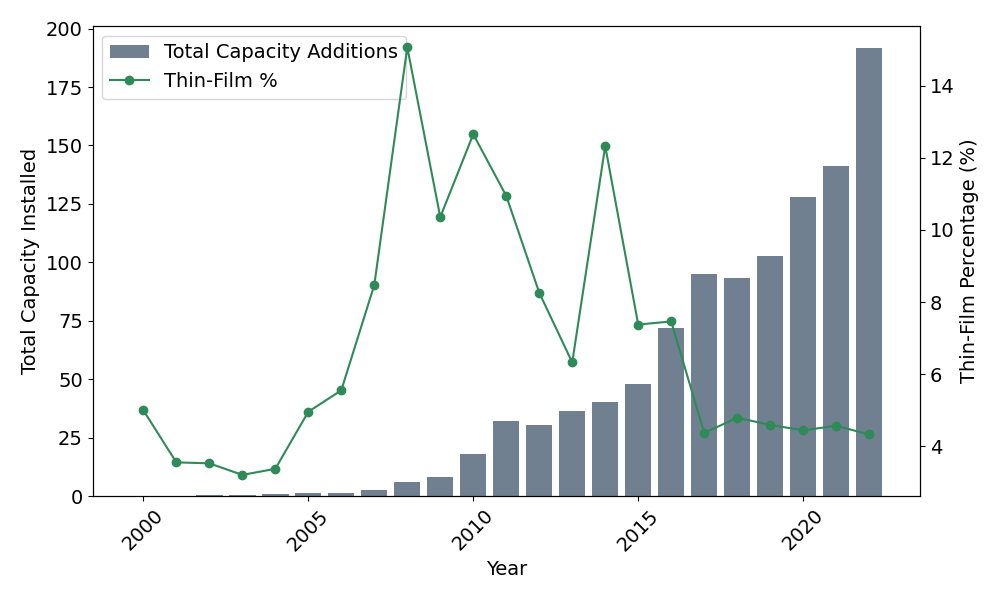
\includegraphics[width=0.5\linewidth]{Figures/ThinFilmPercentageAndCapacity.png}
    \caption{Total Capacity Installed and Thin Film Percentage}
    \label{fig:enter-label}
\end{figure}

\begin{figure}
    \centering
    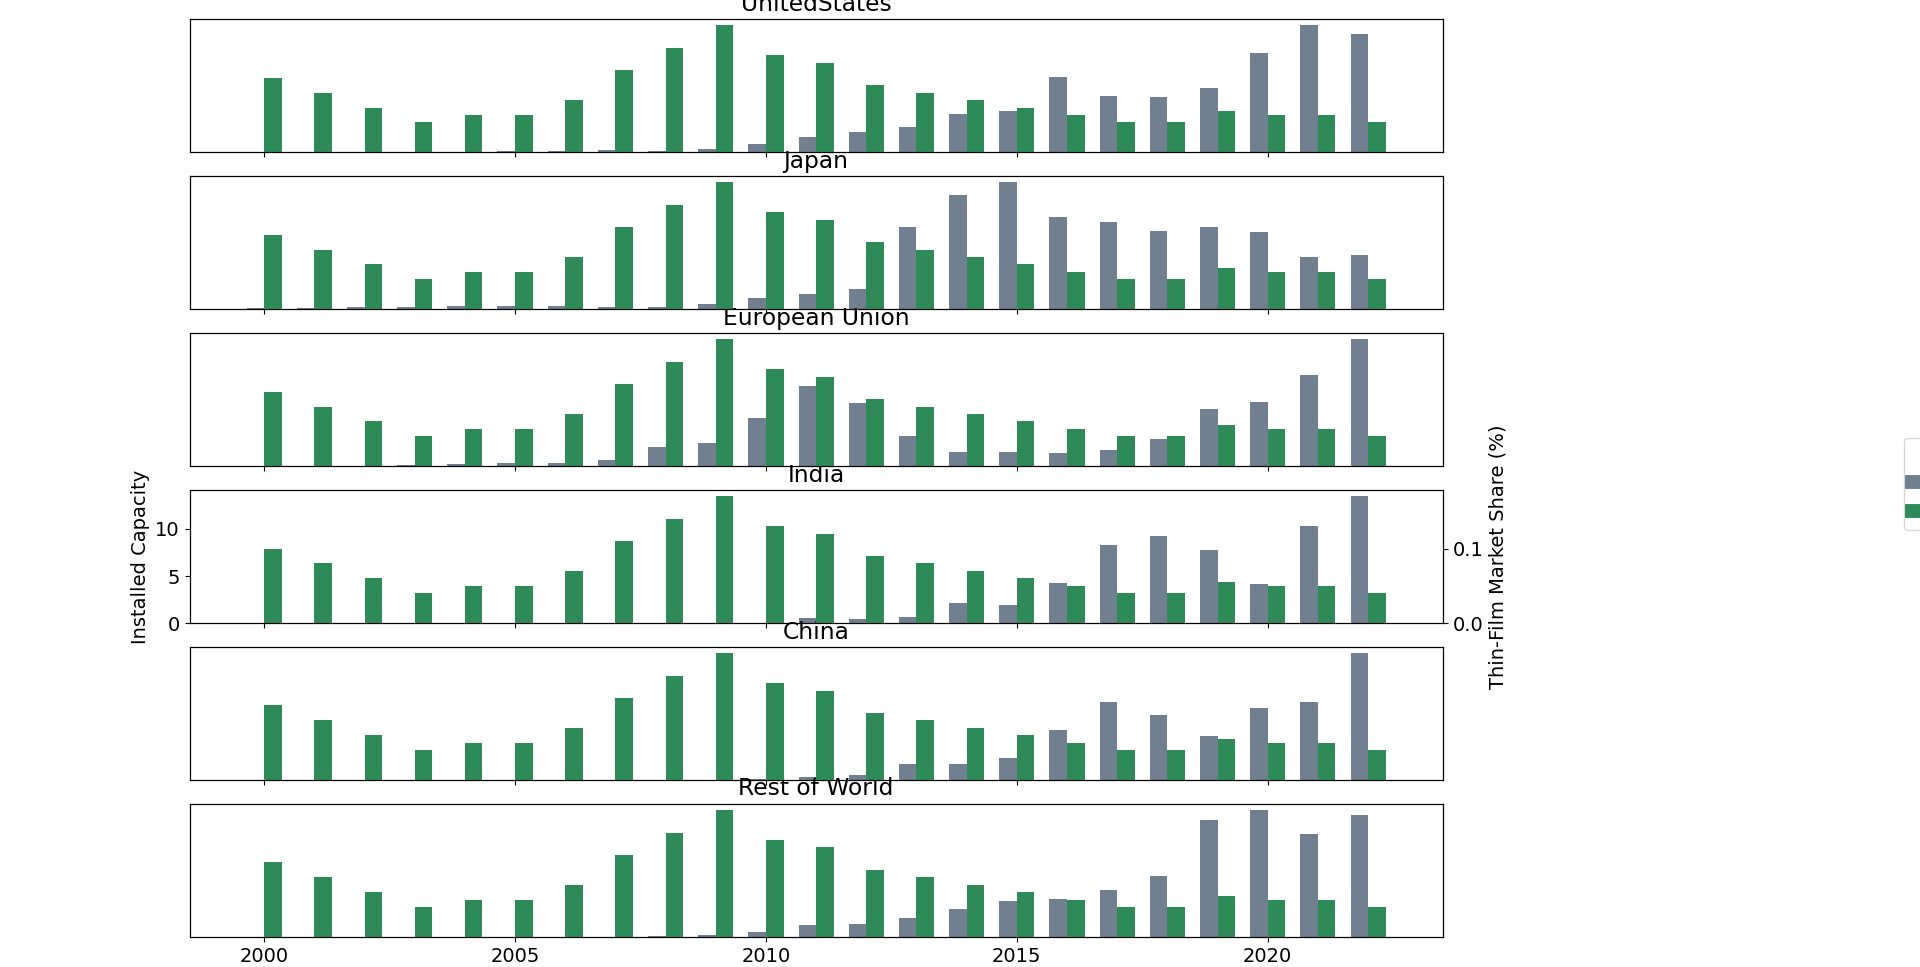
\includegraphics[width=0.5\linewidth]{Figures/Installed Capacity and Thin-film Market Share.png}
    \caption{Total Capacity Installed and Thin Film Percentage by Country}
    \label{fig:enter-label}
\end{figure}

\begin{figure}
    \centering
    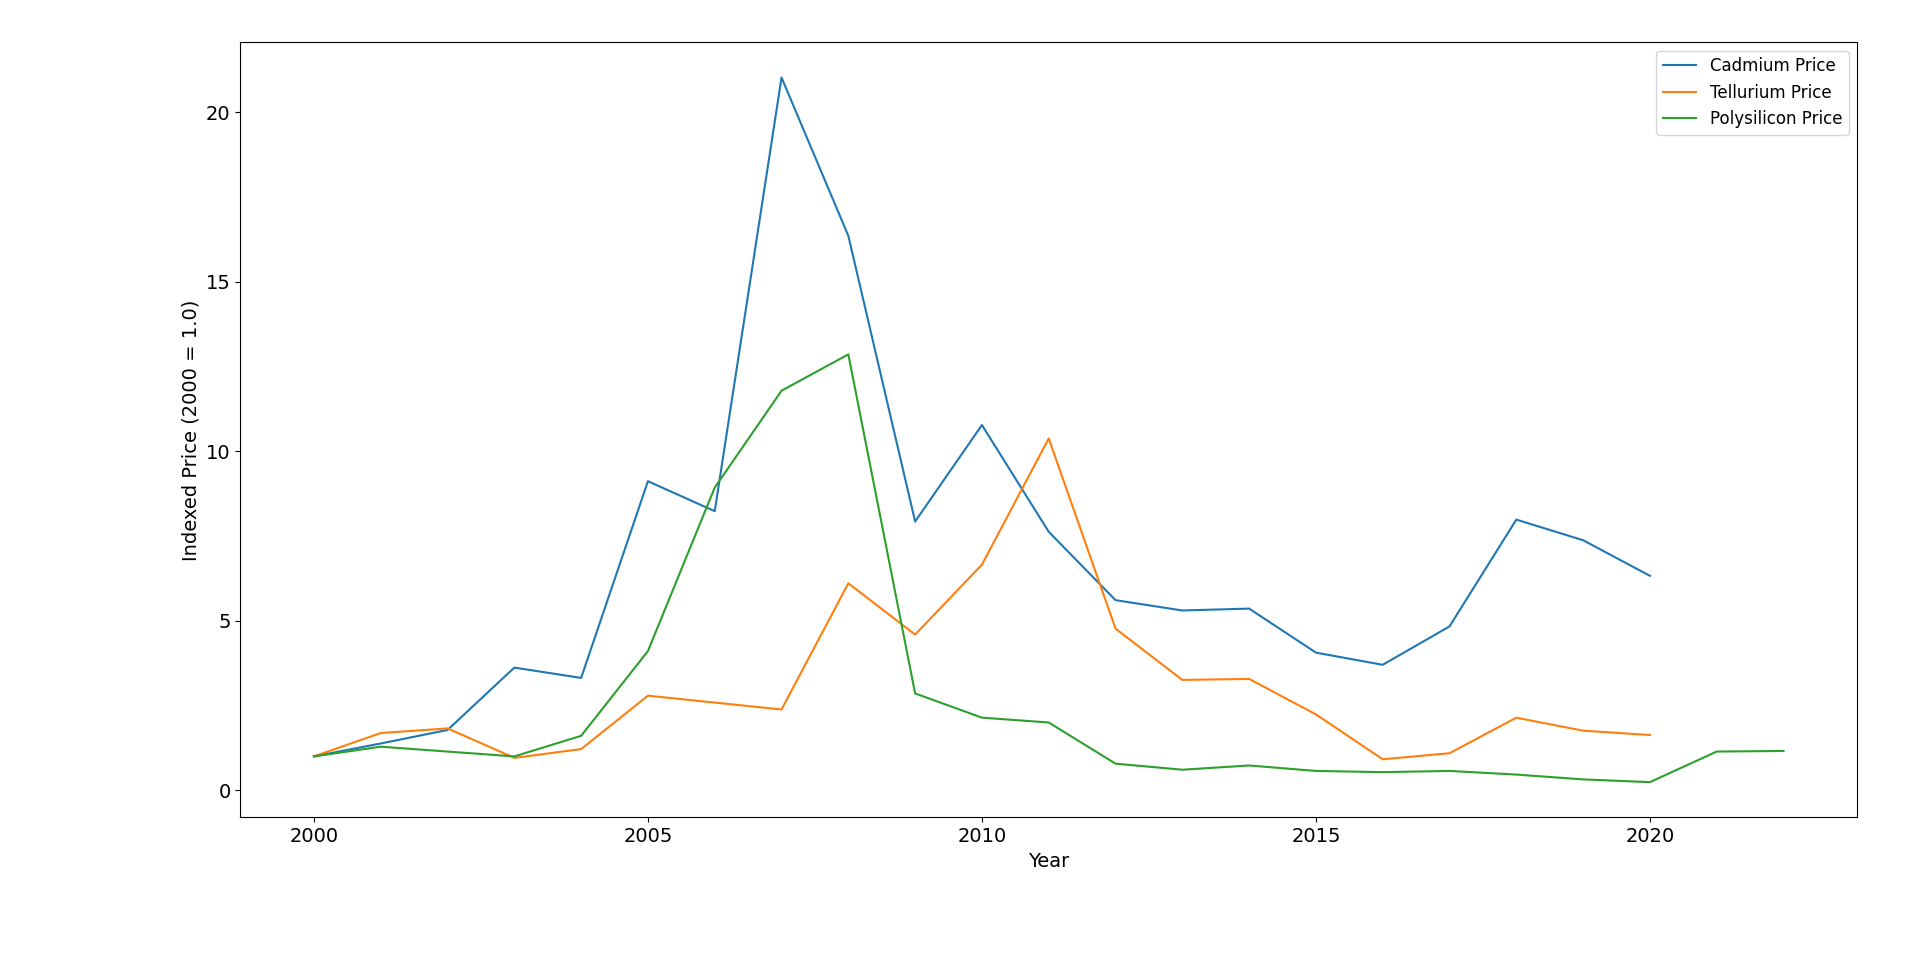
\includegraphics[width=0.5\linewidth]{Figures/Price by Material over Time.png}
    \caption{Price of Input Material by Material Type}
    \label{fig:enter-label}
\end{figure}

\begin{figure}
    \centering
    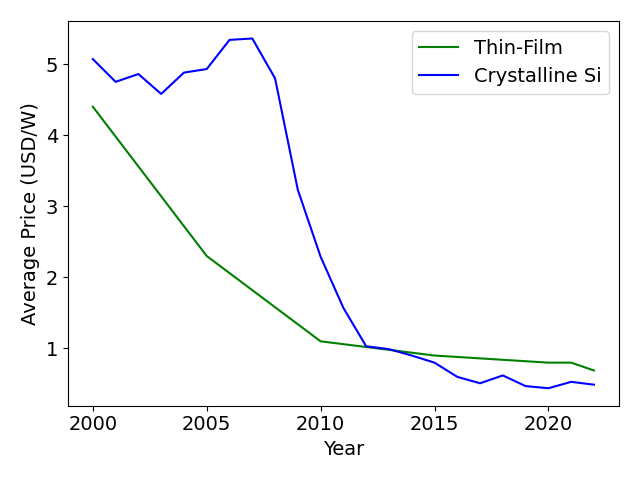
\includegraphics[width=0.5\linewidth]{Figures/Price Per Watt by Technology1.png}
    \caption{Price Per Watt by Technology over Time}
    \label{fig:enter-label}
\end{figure}

\begin{figure}
    \centering
    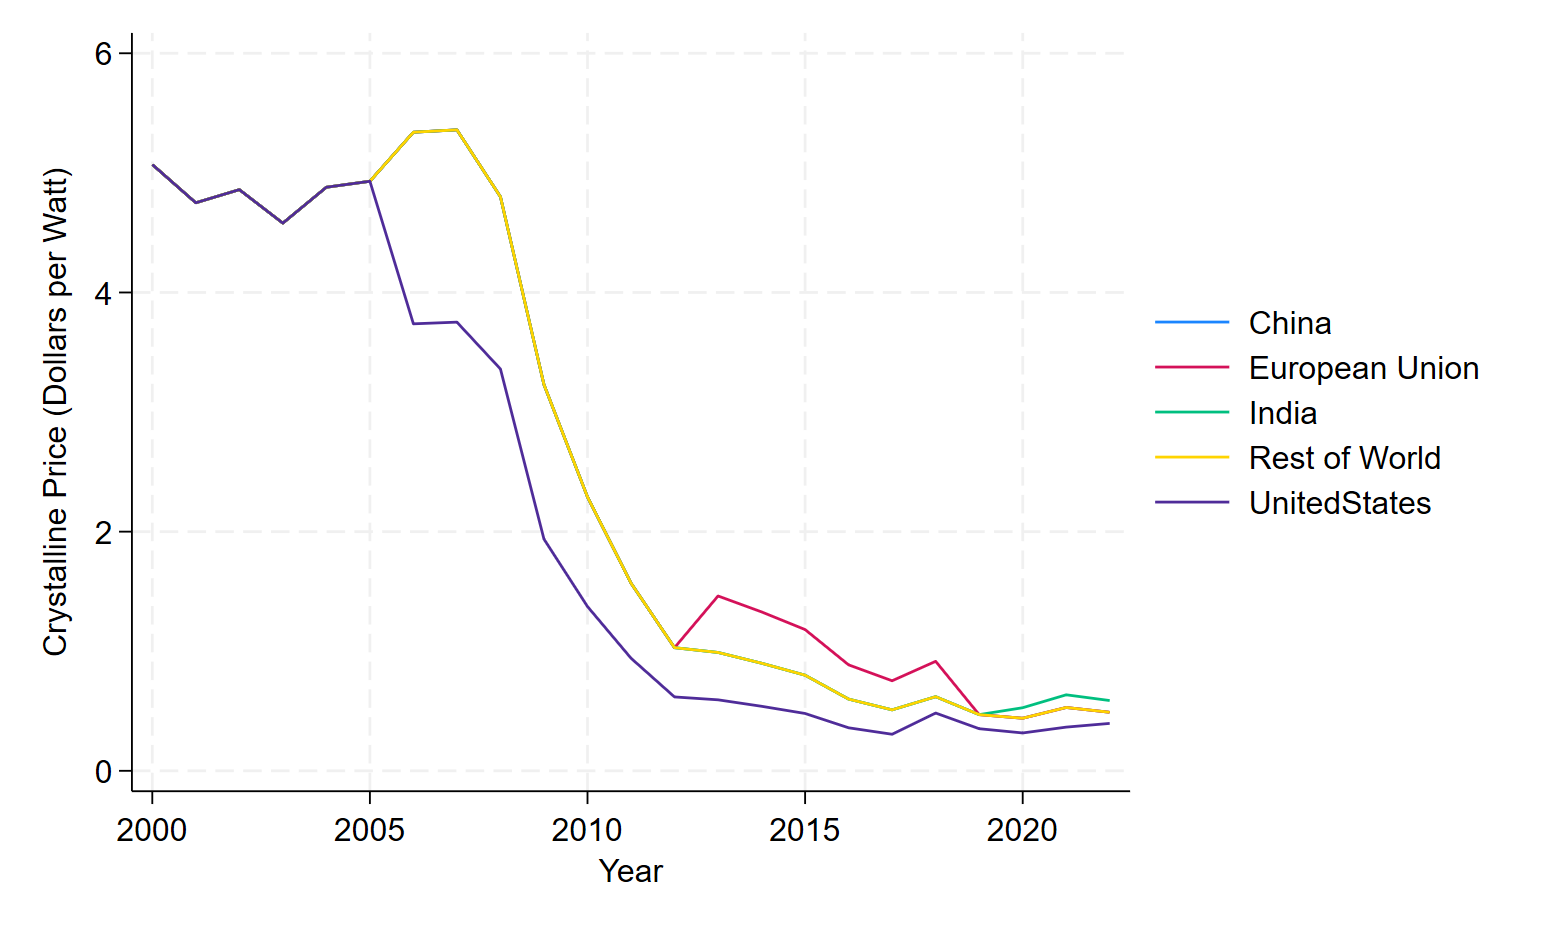
\includegraphics[width=0.5\linewidth]{Figures/CrystallinePriceOverTimebyCountry.png}
    \caption{Crystalline Panel Price over Time by Country}
    \label{fig:enter-label}
\end{figure}


\begin{figure}
    \centering
    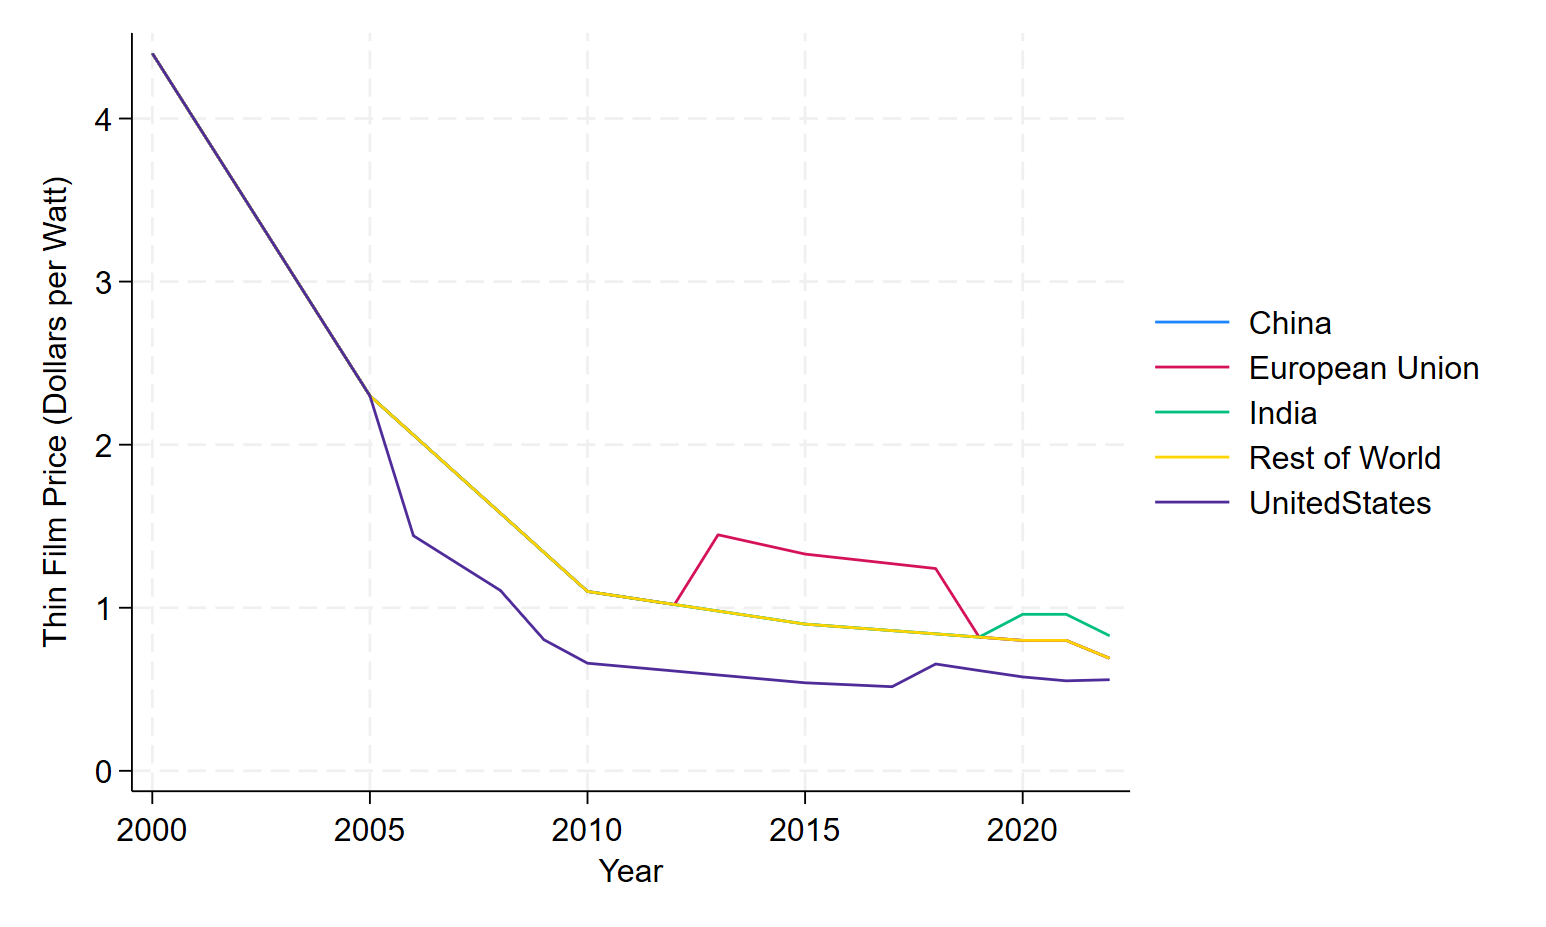
\includegraphics[width=0.5\linewidth]{Figures/ThinFilmPriceOverTimebyCountry.png}
    \caption{Thin-film Price over Time by Country}
    \label{fig:enter-label}
\end{figure}

\begin{figure}
    \centering
    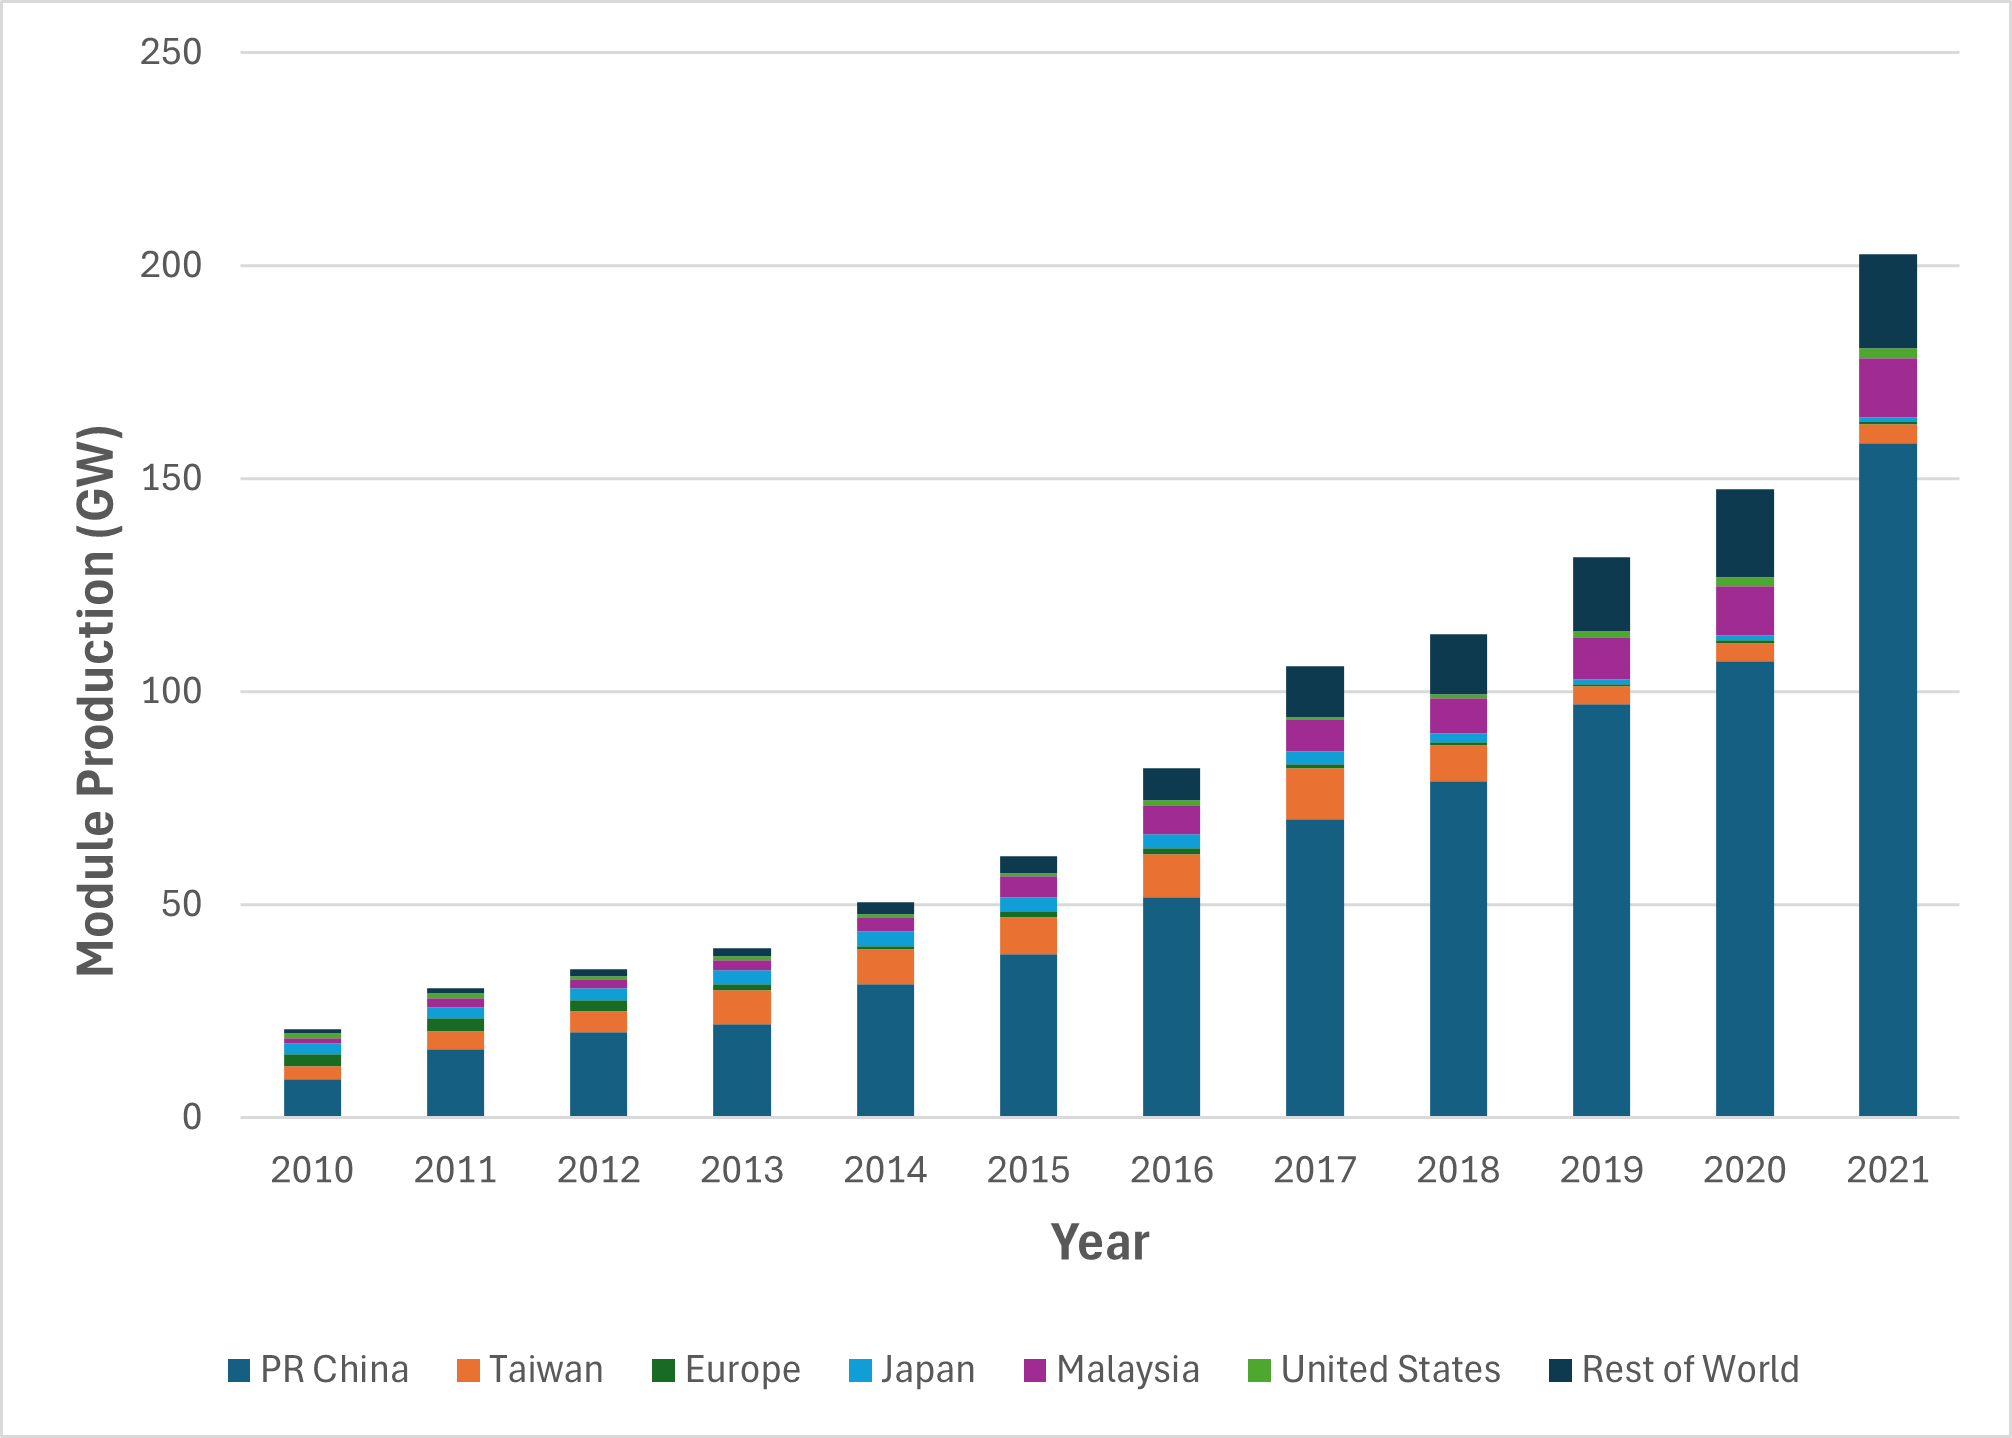
\includegraphics[width=0.5\linewidth]{Figures/ProductionMarketSharebyCountry.png}
    \caption{Total Capacity Installed and Thin Film Percentage}
    \label{fig:enter-label}
\end{figure}


\begin{figure}
    \centering
    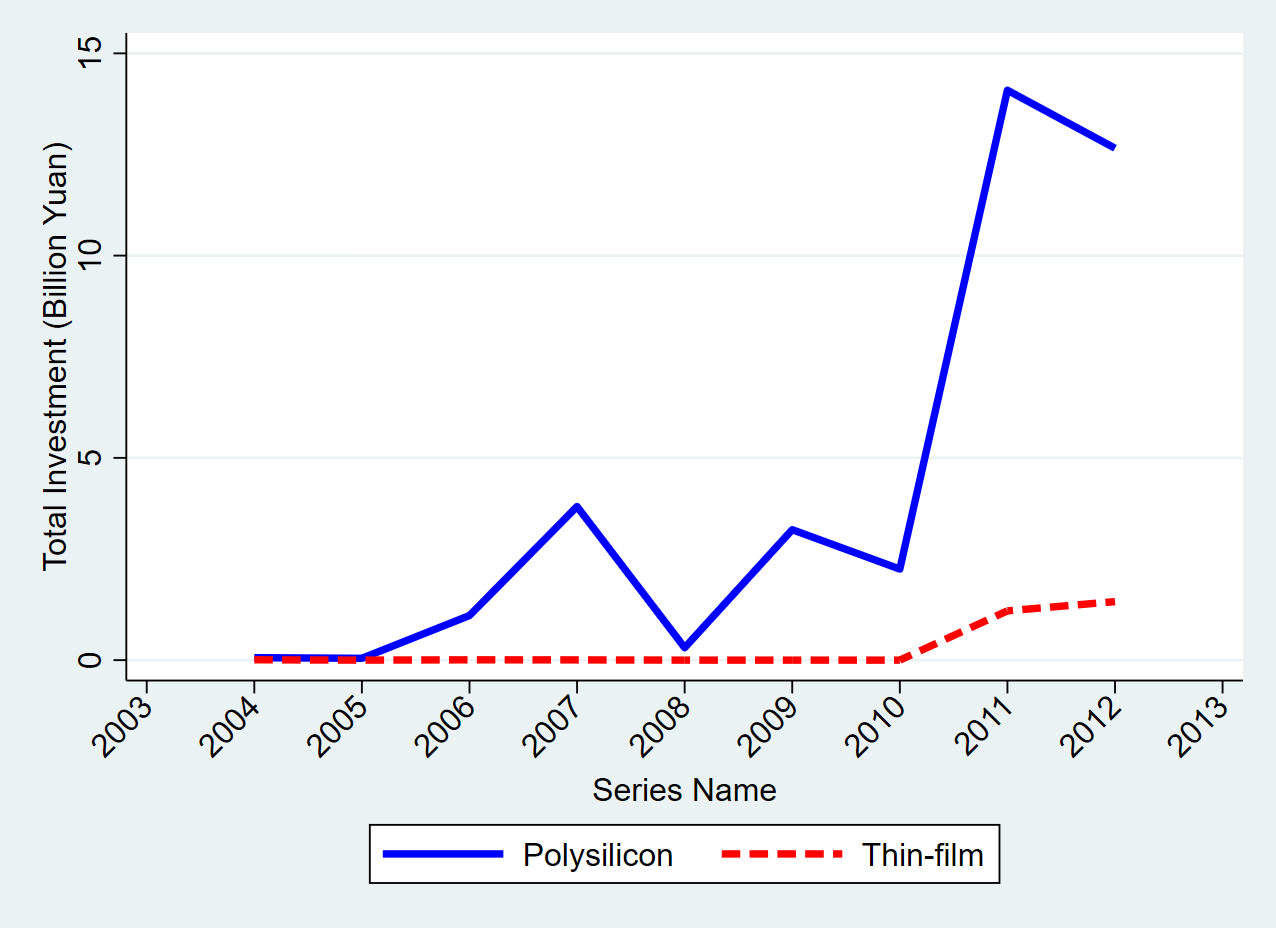
\includegraphics[width=0.5\linewidth]{Figures/InvestmentByFirmType.png}
    \caption{Investment by Firm-type}
    \label{fig:enter-label}
\end{figure}


\begin{figure}
    \centering
    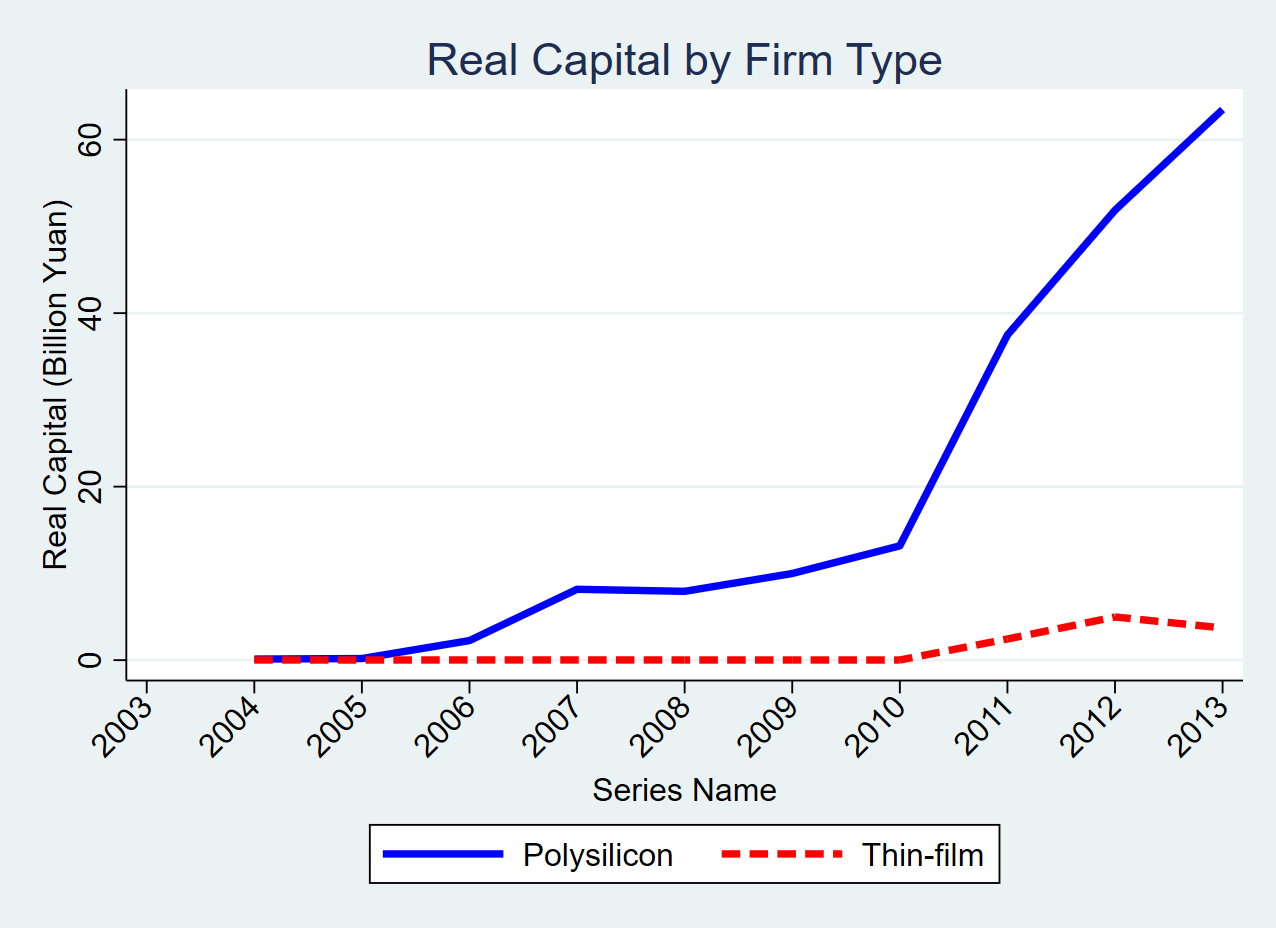
\includegraphics[width=0.5\linewidth]{Figures/RealCapitalByFirmType.png}
    \caption{Capital over Time by Firm Type}
    \label{fig:enter-label}
\end{figure}


\begin{figure}
    \centering
    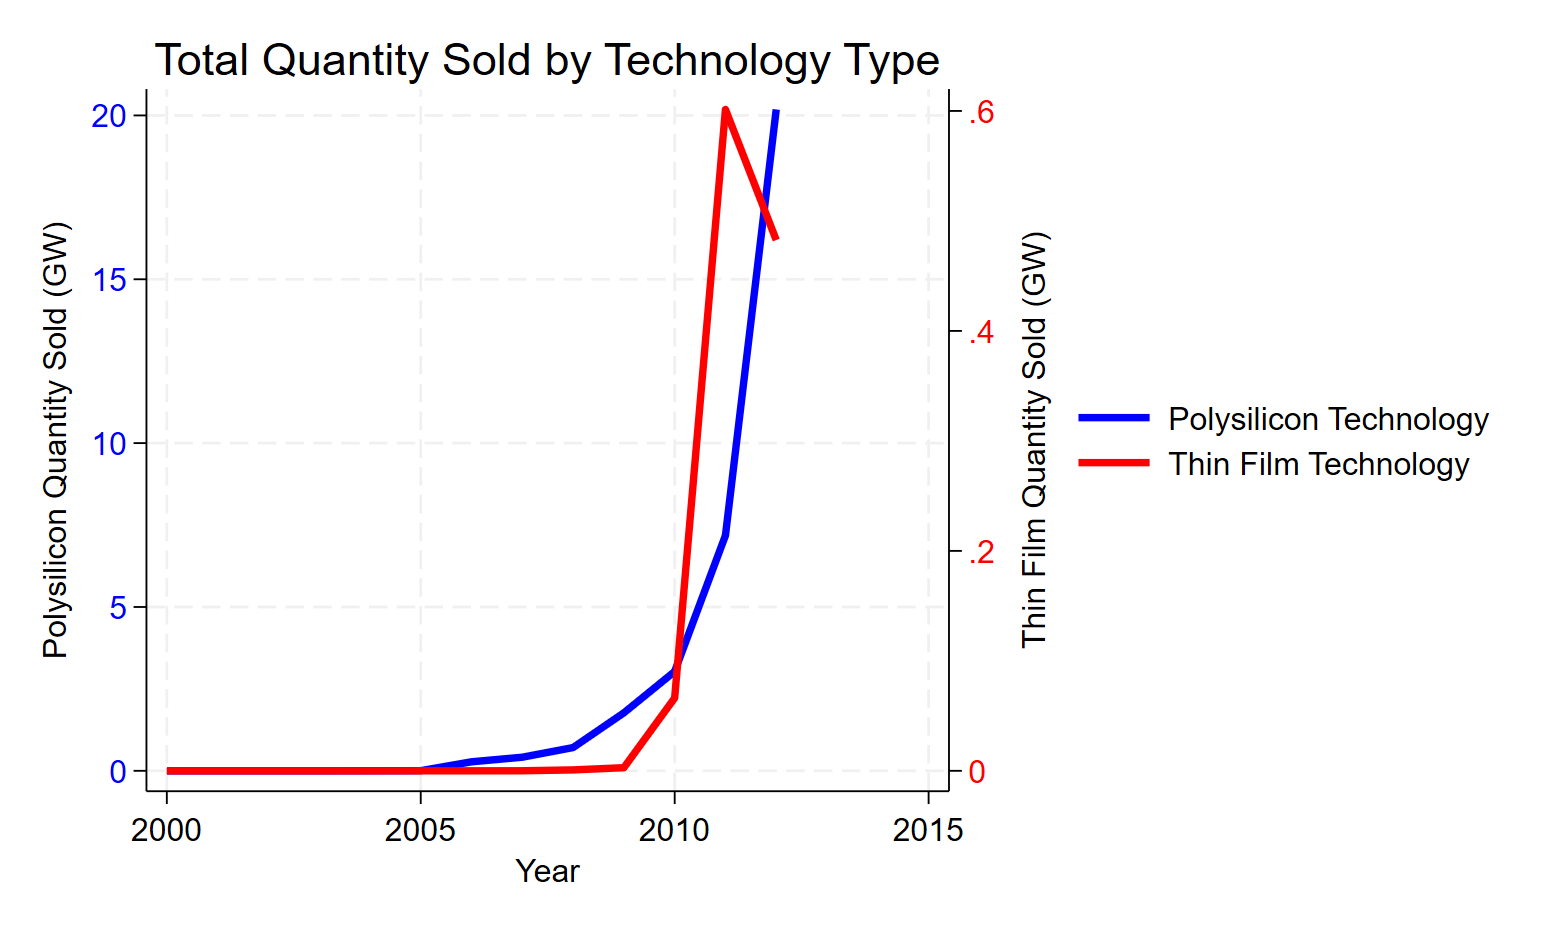
\includegraphics[width=0.5\linewidth]{Figures/QuantitySoldbyTechnologyType.png}
    \caption{Quantity Sold over Time by Technology Type}
    \label{fig:enter-label}
\end{figure}



\begin{figure}
    \centering
    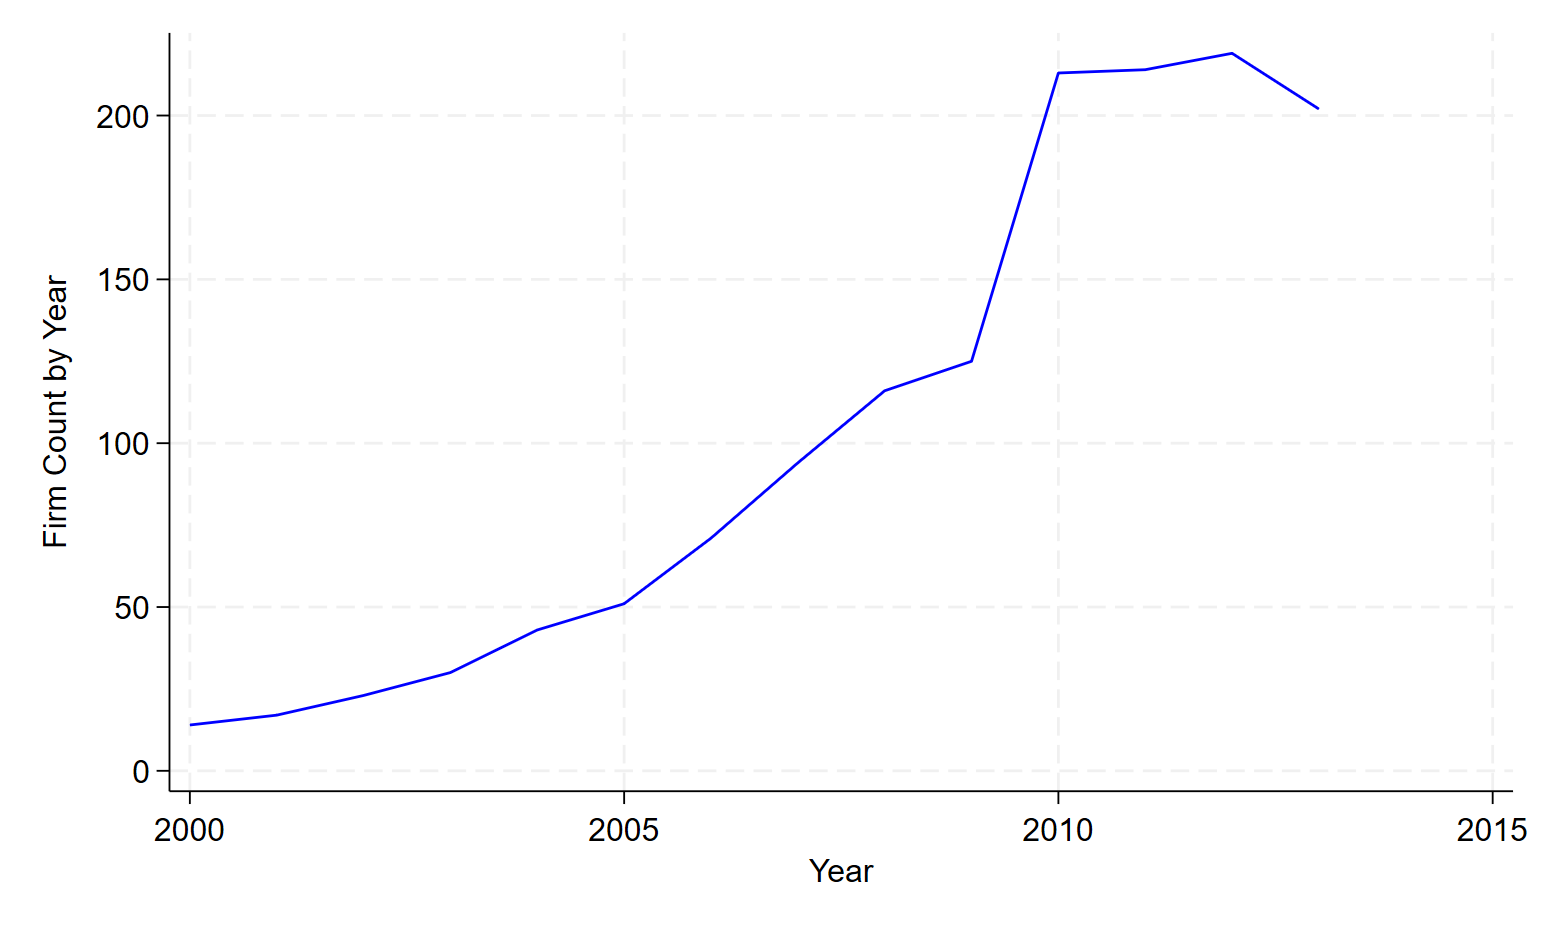
\includegraphics[width=0.5\linewidth]{Figures/FirmCountOverTime.png}
    \caption{Total Firms by Year}
    \label{fig:enter-label}
\end{figure}

\begin{figure}
    \centering
    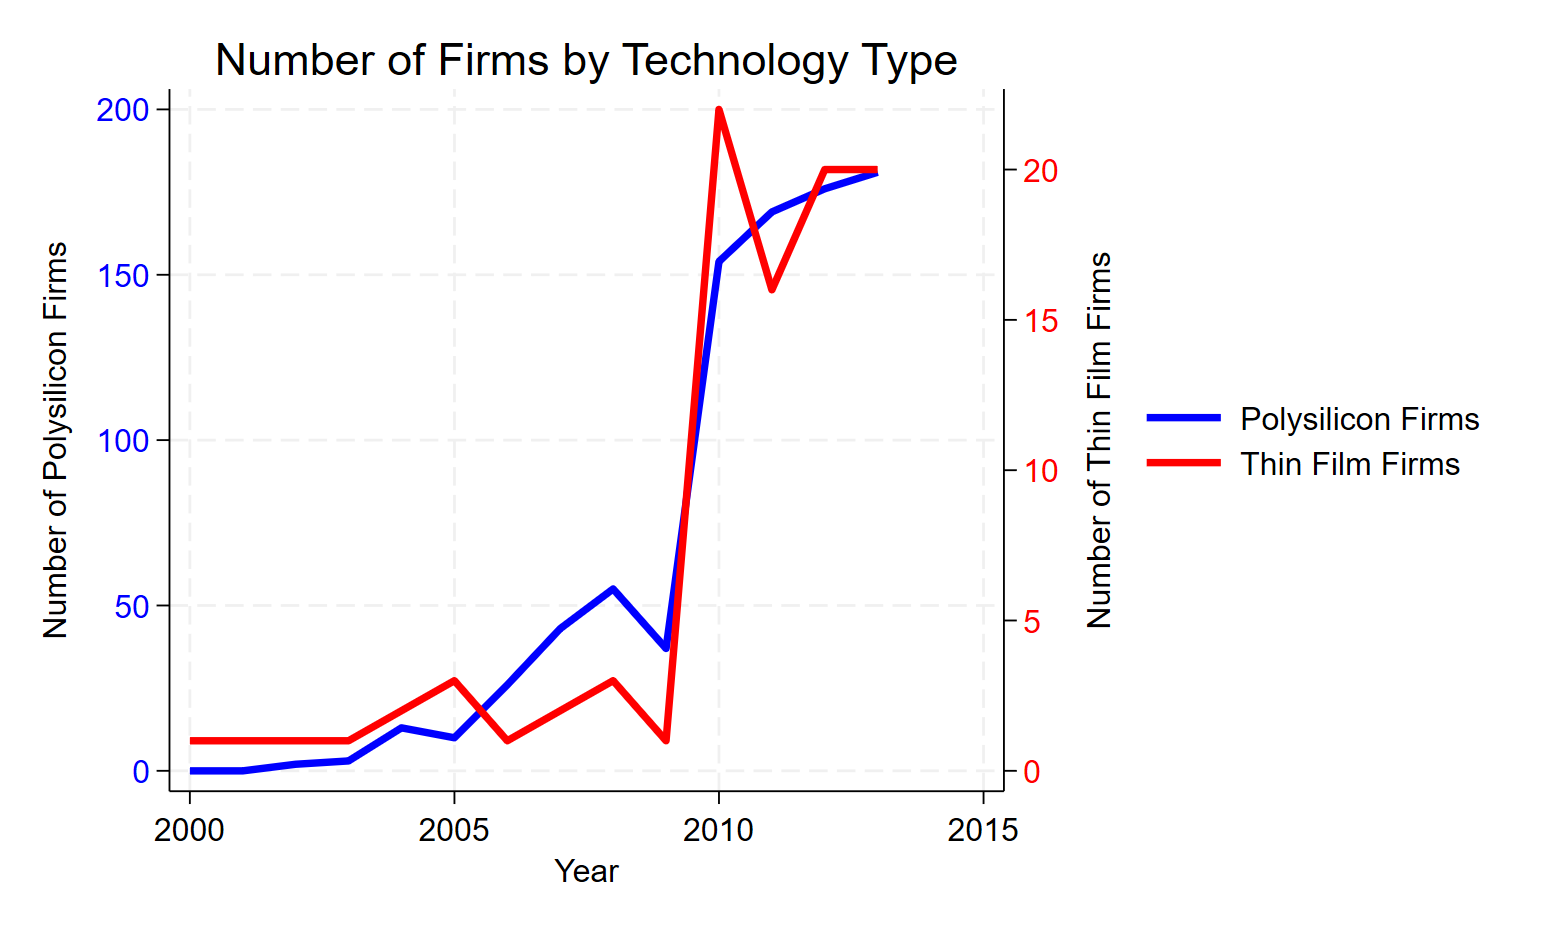
\includegraphics[width=0.5\linewidth]{Figures/FirmCountOverTimebyFirmType.png}
    \caption{Total Firms by Year and Firm Type}
    \label{fig:enter-label}
\end{figure}

\begin{figure}
    \centering
    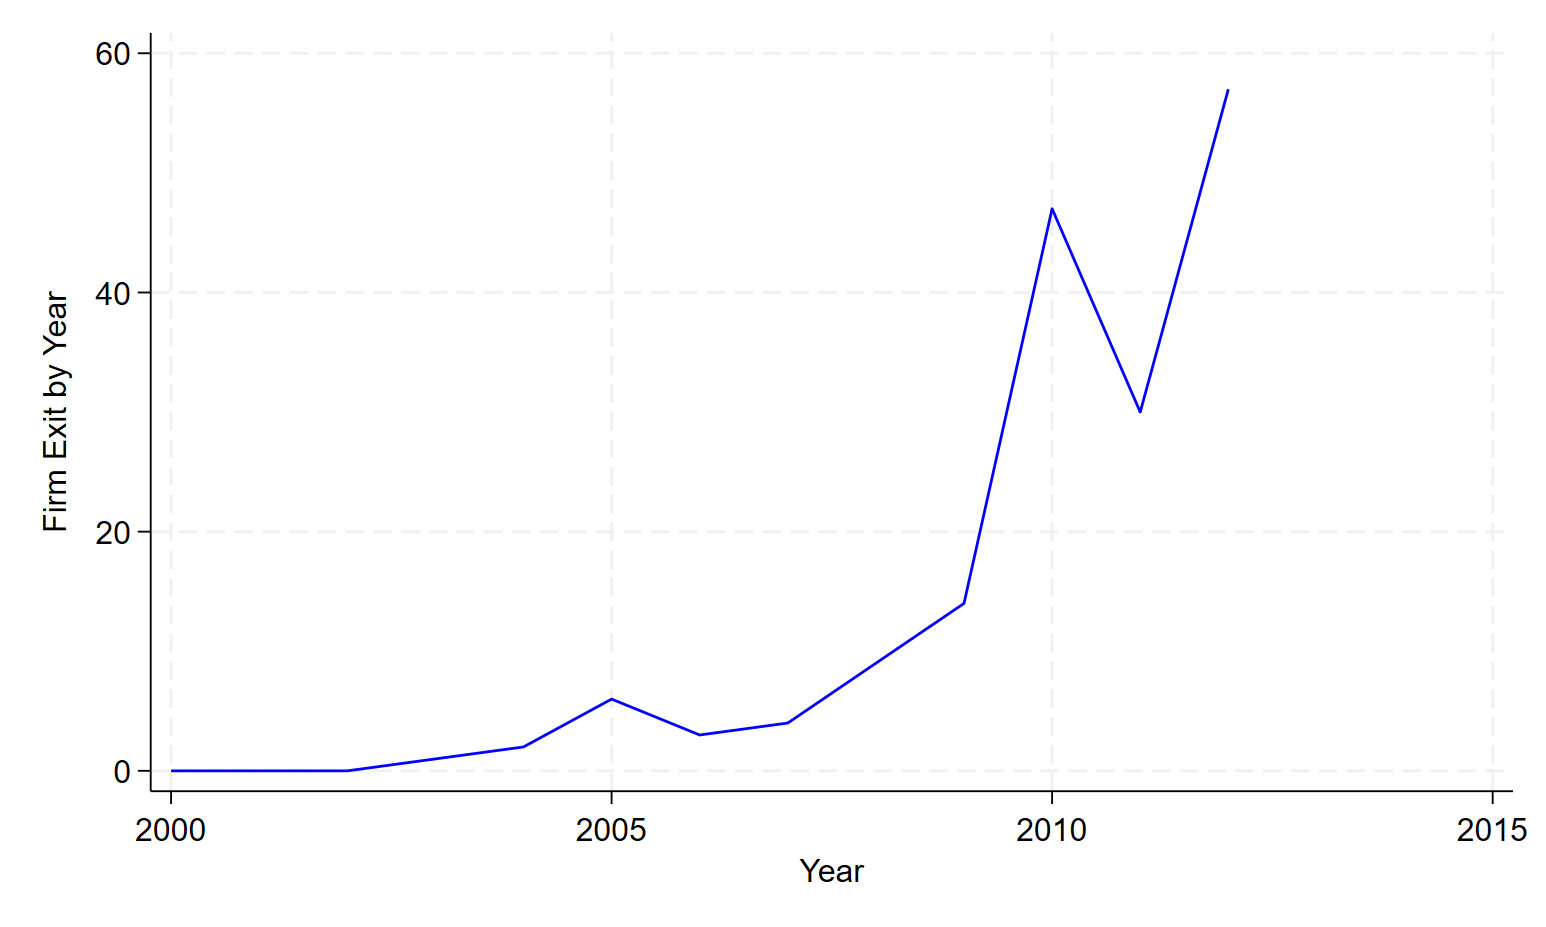
\includegraphics[width=0.5\linewidth]{Figures/FirmExitOverTime.png}
    \caption{Firm Exits by Year}
    \label{fig:enter-label}
\end{figure}

\begin{figure}
    \centering
    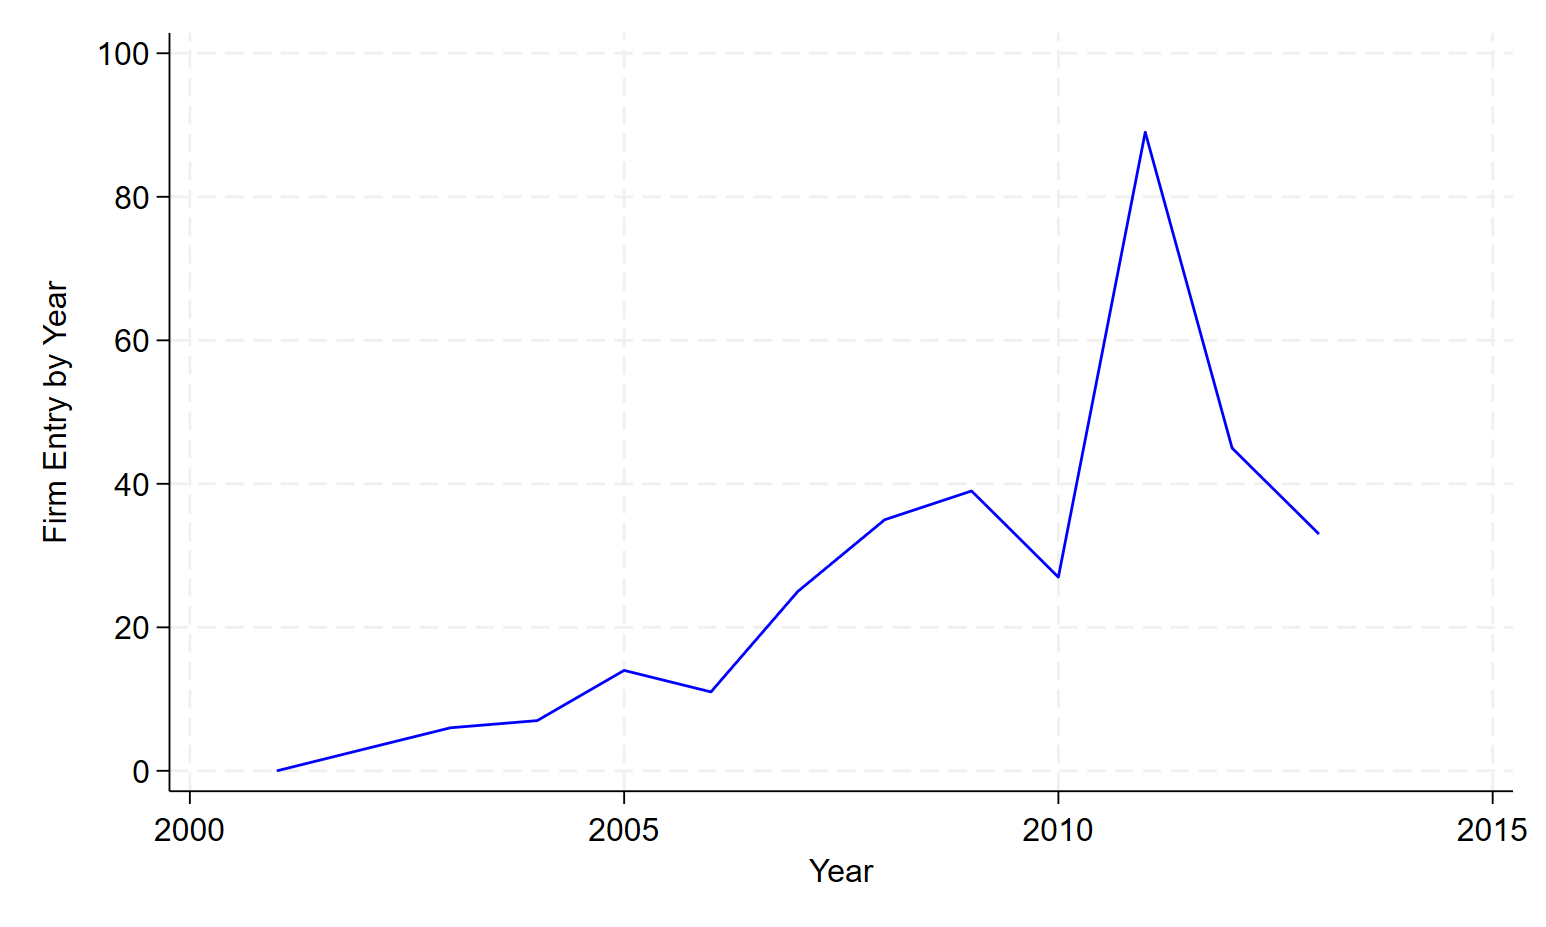
\includegraphics[width=0.5\linewidth]{Figures/FirmEntryOverTime.png}
    \caption{Firm Entry by Year}
    \label{fig:enter-label}
\end{figure}



\end{document}